% \PassOptionsToPackage{quiet}{fontspec} % 抑制中文字体警告
\documentclass[aspectratio=169]{beamer}
\usepackage[UTF8]{ctex}
\usepackage[T1]{fontenc}

\usepackage{hyperref}
% other packages
\usepackage{latexsym,amsmath,xcolor,multicol,booktabs,calligra}
\usepackage{graphicx,pstricks,listings,stackengine}

\counterwithin{equation}{section} %公式按照章节编号

% defs
\def\cmd#1{\texttt{\color{red}\footnotesize $\backslash$#1}}
\def\env#1{\texttt{\color{blue}\footnotesize #1}}
\definecolor{deepblue}{rgb}{0,0,0.5}
\definecolor{deepred}{rgb}{0.6,0,0}
\definecolor{deepgreen}{rgb}{0,0.5,0}
\definecolor{halfgray}{gray}{0.55}
\lstset{
    basicstyle=\ttfamily\small,
    keywordstyle=\bfseries\color{deepblue},
    emphstyle=\ttfamily\color{deepred},    % Custom highlighting style
    stringstyle=\color{deepgreen},
    numbers=left,
    numberstyle=\small\color{halfgray},
    rulesepcolor=\color{red!20!green!20!blue!20},
    frame=shadowbox,
}
\usepackage{xjut}
\setbeamertemplate{background}{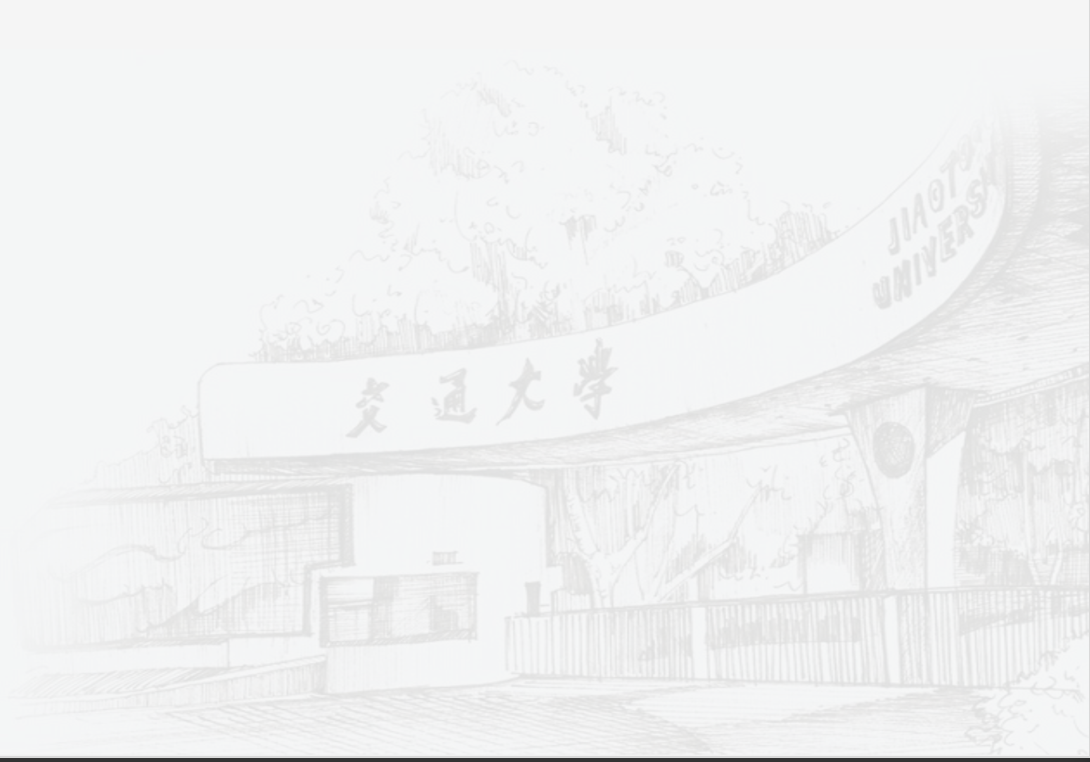
\includegraphics[width=\paperwidth]{xjtu/xjut_draw.png}}

\AtBeginSection[]{
	\begin{frame}
        \begin{columns}
            \begin{column}{.45\textwidth}
                \tableofcontents[sections=1-4,sectionstyle=show/shaded,subsectionstyle=show/shaded/hide,subsubsectionstyle=show/shaded/hide]
            \end{column}
            \begin{column}{.45\textwidth}
                \tableofcontents[sections=5-8,sectionstyle=show/shaded,subsectionstyle=show/shaded/hide,subsubsectionstyle=show/shaded/hide]
            \end{column}
        \end{columns}
	\end{frame}
}

\usefonttheme[onlymath]{serif}

\title{无人机遂行编队飞行中的纯方位无源定位}
\author{徐翌森}
\institute{软件2204}
\date{\today}

\begin{document}

\begin{frame}
    \titlepage
    \begin{figure}[h]
        \centering
        
\includegraphics[width=0.15\textwidth]{xjtu/XJUT_Logo.png}
    \end{figure}
\end{frame}

%%%%%%%%%%%%%%%%%%%%%%%%%%%%%%%%%%%%%%%%%%%%%%%%%%%%%%%%%%%%%%%%
%                                                              %
%%%%%%%%%%%%%%%%%%%%%%%%%%%%%%%%%%%%%%%%%%%%%%%%%%%%%%%%%%%%%%%%

\section{问题重述}
\begin{frame}{问题背景}

在现代无人机编队飞行任务中,为最大化隐蔽性和安全性,无人机群体需尽量减少向外界发射电磁波信号,以避免被敌方探测。所以需要在保持电磁静默的同时,确保无人机能够准确维持或调整至正确的编队位置。

因此题目要求我们,开发一种纯方位无源定位方法,通过编队内部部分无人机发射信号,其余无人机被动接收信号并根据接收到的方向信息进行自我位置调整,以实现编队飞行中的精确定位与队形保持。
\end{frame}


\begin{frame}{问题一}
    \begin{columns}
        \column{0.45\textwidth}
        \begin{figure}[!ht]
            \centering
            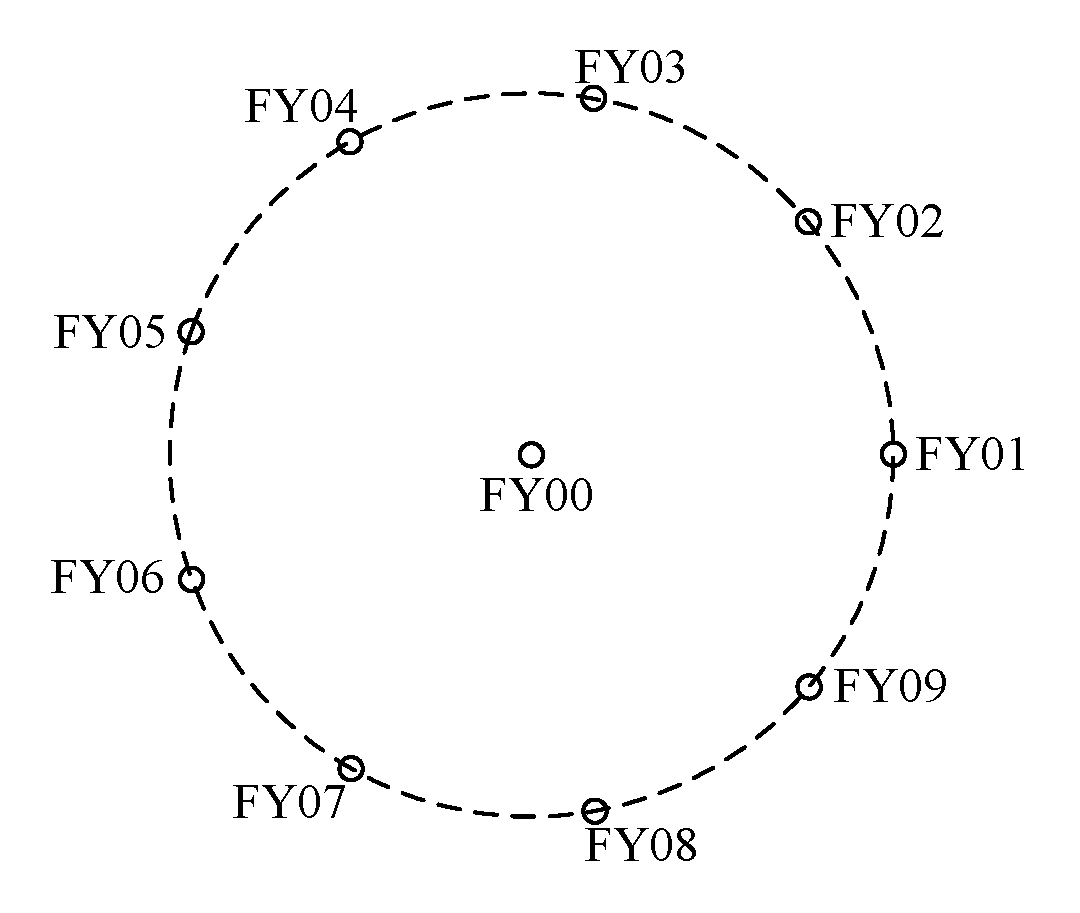
\includegraphics[width=\textwidth]{图片/无人机以及编号示意图.pdf}
        \end{figure}
        \column{0.55\textwidth}
        对于左图所示的圆形的无人机队列,题目要求我们完成如下要求:
        \begin{itemize}
            \item 基于圆心无人机和圆周上两架无人机发射的信号,建立接收信号的无人机的定位模型;
            \item 探究除FY00和FY01外,如果其他发射信号的无人机编号未知,最少几架无人机发射信号可以确定接收信号的无人机的位置;
            \item 对于初始未知略有偏差的情况,给出无人机位置的调整方案。
        \end{itemize}
    \end{columns}
\end{frame}

\begin{frame}{问题二}
    \begin{columns}
        \column{0.45\textwidth}
        \begin{figure}[!ht]
            \centering
            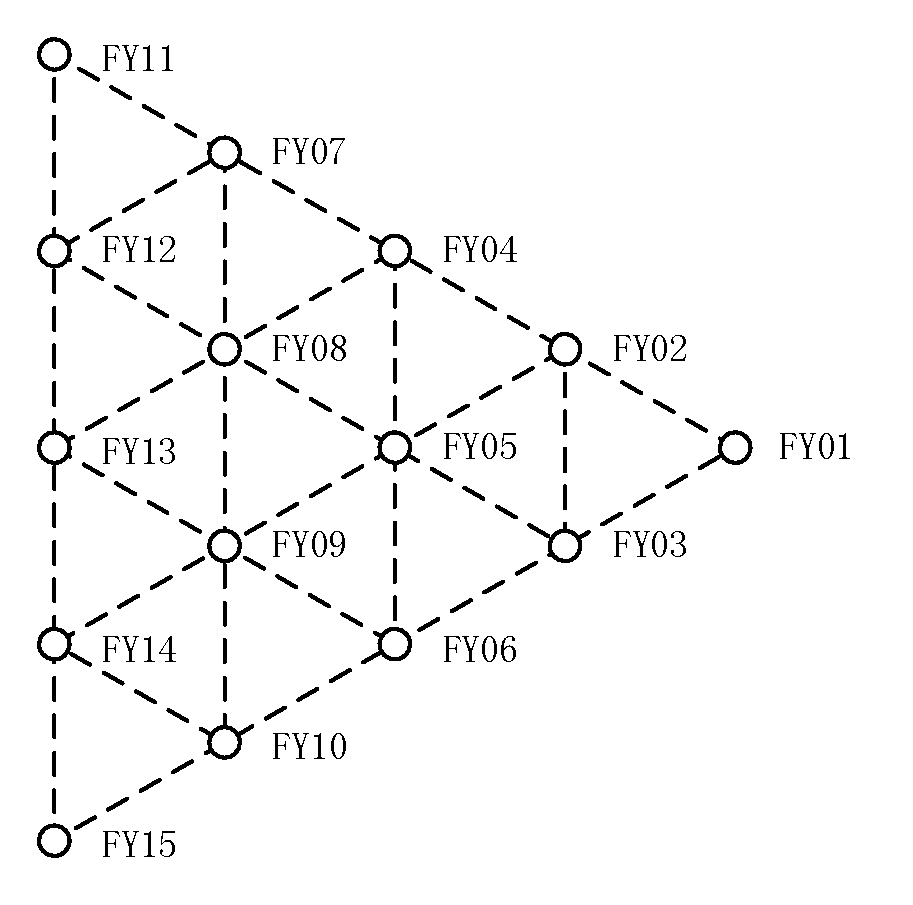
\includegraphics[width=0.8\textwidth]{图片/锥形队列.pdf}
        \end{figure}
        \column{0.55\textwidth}
        接下来,对于左图所示的锥形无人机队列。题目要求我们仍然考虑无源定位的情况,并给出调整方案。
    \end{columns}
\end{frame}

%%%%%%%%%%%%%%%%%%%%%%%%%%%%%%%%%%%%%%%%%%%%%%%%%%%%%%%%%%%%%%%%
%                                                              %
%%%%%%%%%%%%%%%%%%%%%%%%%%%%%%%%%%%%%%%%%%%%%%%%%%%%%%%%%%%%%%%%

\section{基本假设}

\begin{frame}{基本假设}
    我们有如下的基本假设:
    \begin{itemize}
        \item 无人机之间的信息不能共享;
        \item 发射信号的无人机不能同时接收信号;
        \item 每一架无人机都知道自己的编号;
        \item 每一架无人机都知道不同编号无人机的相对位置关系;
        \item 除特殊要求外(问题一第2小问),接收信号的无人机知道每一个接收的角度信息来源于哪两架无人机;
        \item 在以FY00为原点的极坐标系中,圆周上无人机的极角偏差小于$\frac{1}{18}\pi$;
        \item 无人机只能接收角度信息,也只能依靠角度的信息来引导自己的移动,其基本移动模式为,接收两个角度信号,保持一个角度不变,调整自身位置使得另一个角度为目标数值;
    \end{itemize}
\end{frame}

%%%%%%%%%%%%%%%%%%%%%%%%%%%%%%%%%%%%%%%%%%%%%%%%%%%%%%%%%%%%%%%%
%                                                              %
%%%%%%%%%%%%%%%%%%%%%%%%%%%%%%%%%%%%%%%%%%%%%%%%%%%%%%%%%%%%%%%%

\section{符号说明}

\begin{frame}{符号说明}
    常用符号说明如下表所示:
    \begin{table}[!ht]
        \centering
        \begin{tabular}{cc}
            \toprule
            符号  &  符号说明\\
            \midrule
            $r_0$ & 无人机编队的圆半径\\
            FY0N  & 序号为$n$的无人机\\
            $\alpha_{ABC}$ & FY0B接收的来自于FY0A和FY0C的角信号\\
            $\theta_{ABC}$ & FY0A、FY0B、FY0C三点共圆的圆心极角\\
            $\rho_{ABC}$ & FY0A、FY0B、FY0C三点共圆的圆心极径\\
            $d_{i}$ & FY0I当前位置与正确位置间的距离\\
            \bottomrule
        \end{tabular}
    \end{table}
\end{frame}

%%%%%%%%%%%%%%%%%%%%%%%%%%%%%%%%%%%%%%%%%%%%%%%%%%%%%%%%%%%%%%%%
%                                                              %
%%%%%%%%%%%%%%%%%%%%%%%%%%%%%%%%%%%%%%%%%%%%%%%%%%%%%%%%%%%%%%%%

\section[问题1-1]{问题一(1)接受信号无人机的定位模型}

\subsection{基于两圆相交的定位模型}

\begin{frame}{基于两圆相交的定位模型}
    \begin{columns}
        \column{0.4\textwidth}
        \begin{figure}[!ht]
            \centering
            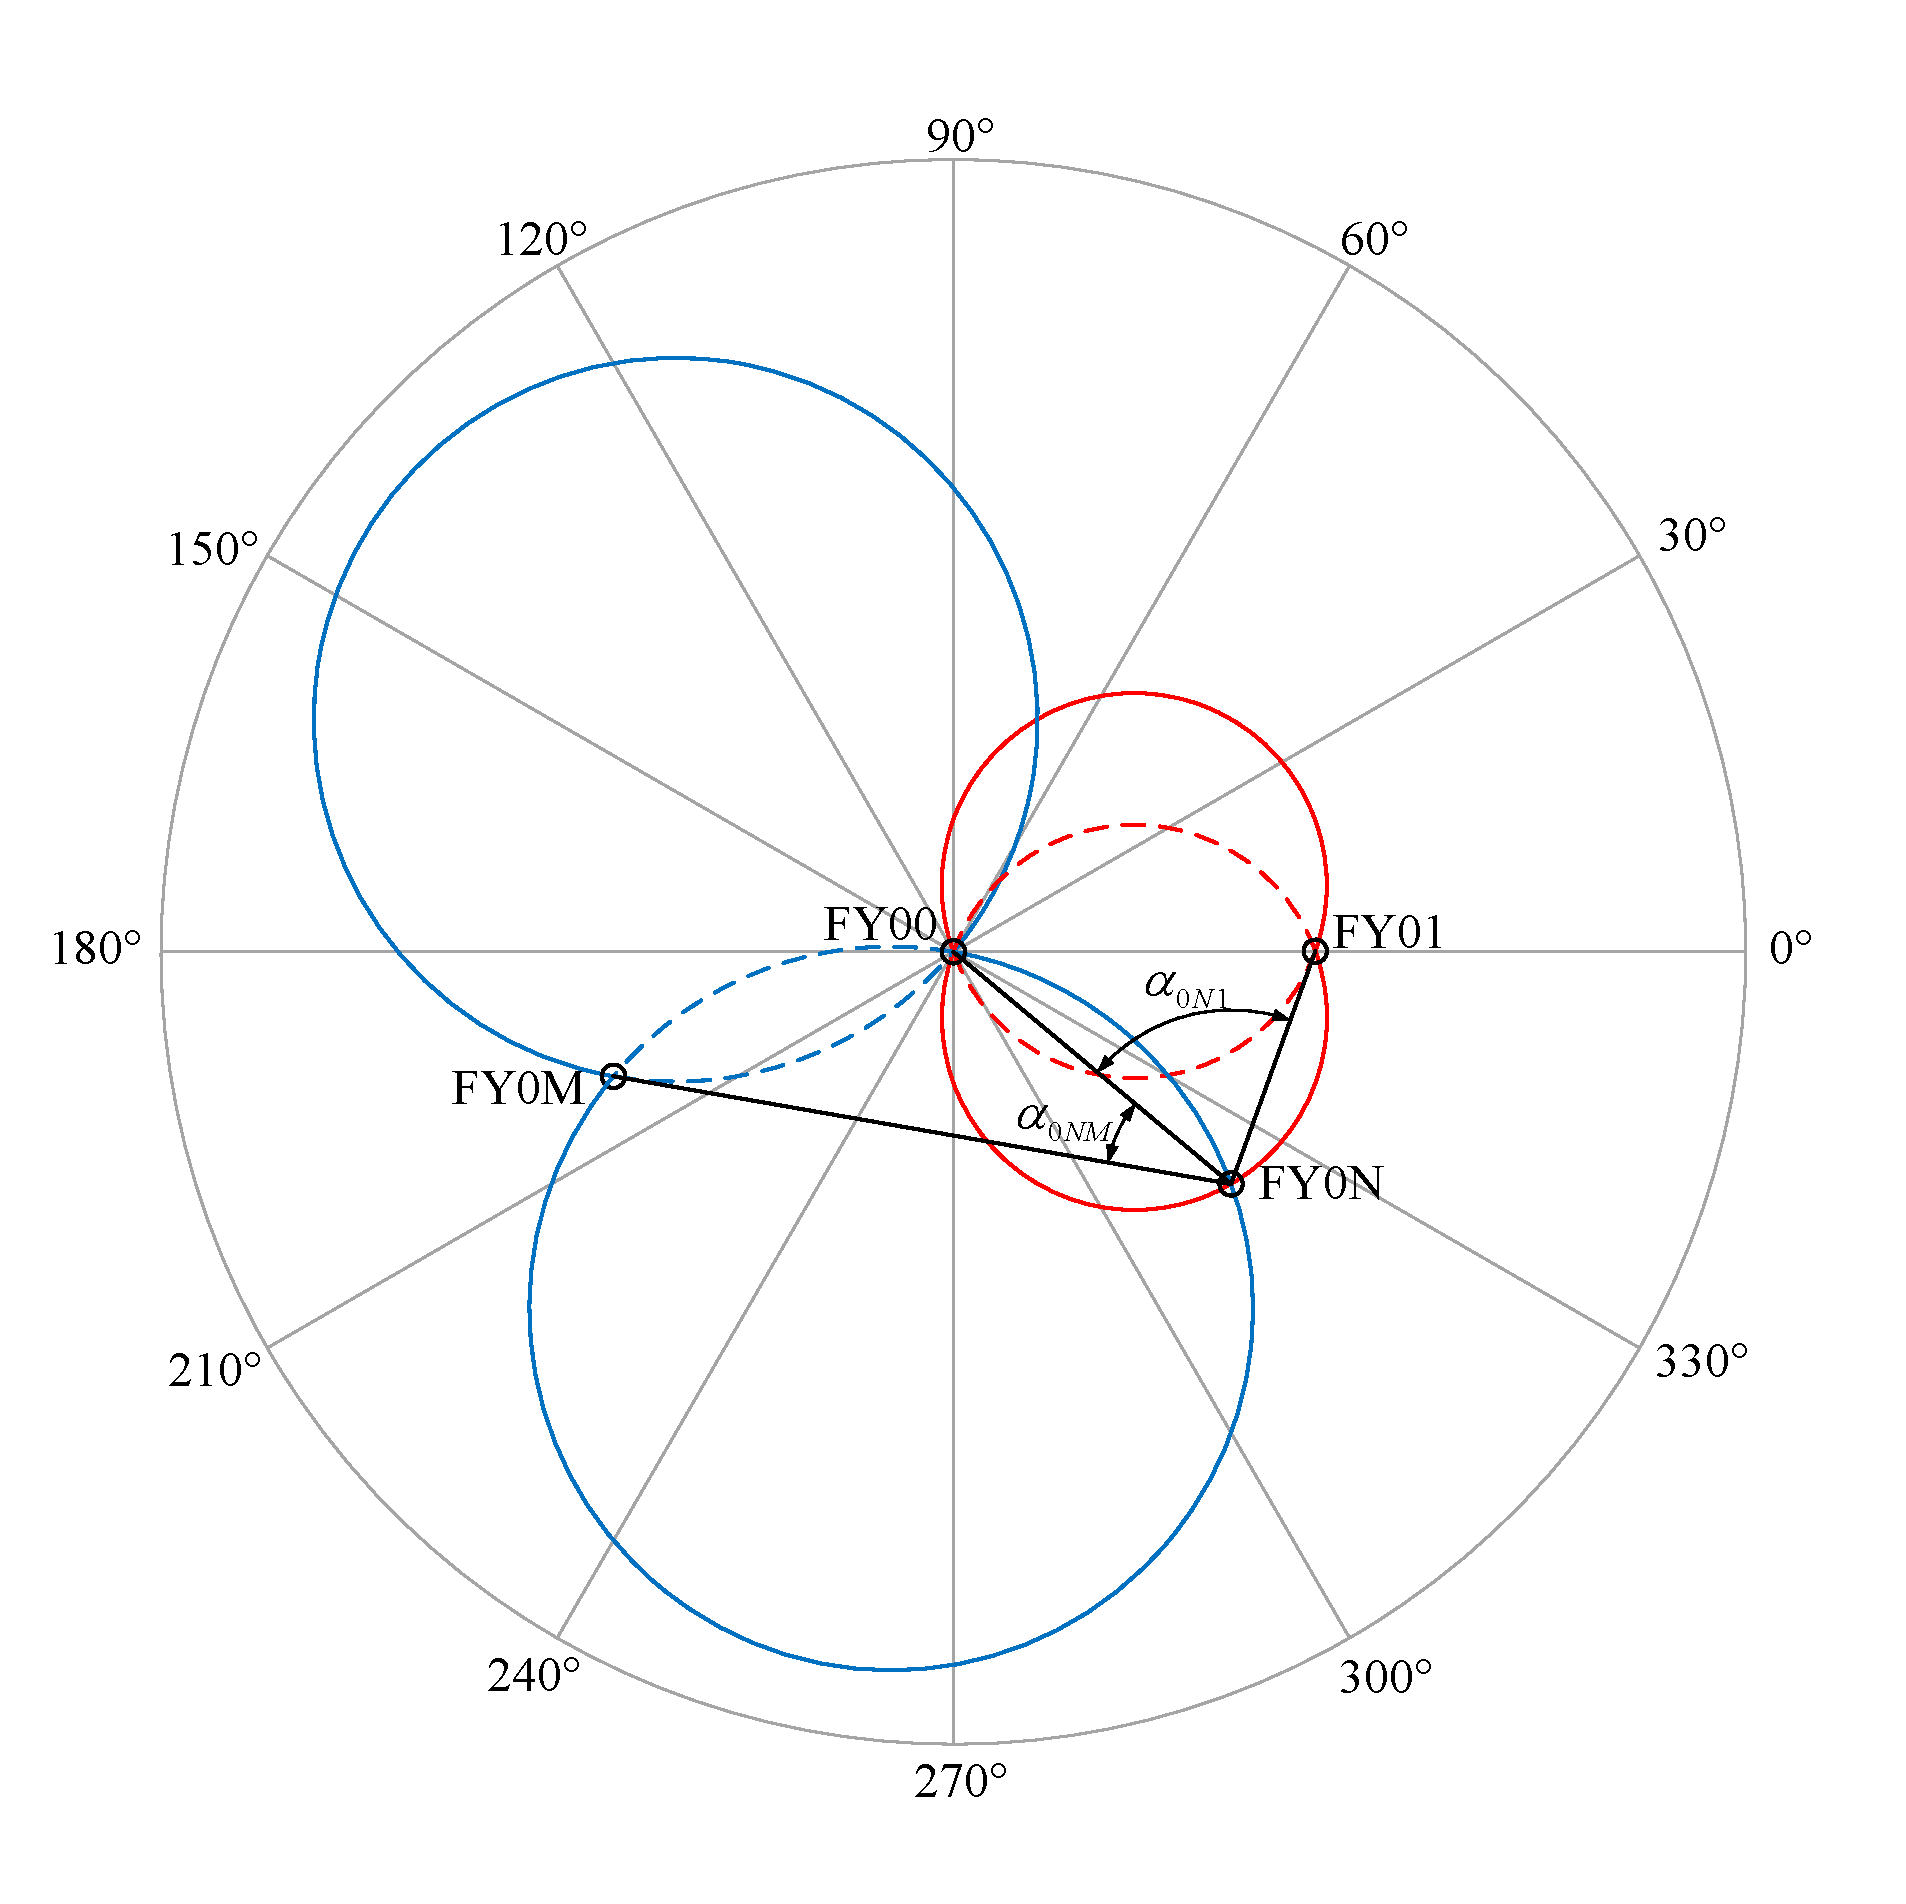
\includegraphics[width=\textwidth]{图片/问题1-1示意图.pdf}
        \end{figure}
        \column{0.6\textwidth}
        由于圆的对称性,我们不妨设其中一个发射信号的无人机为FY01。如左图所示,位于圆心的FY00、位于圆周的FY01和另一架位于圆周但序数任意的无人机FY0M发射信号,FY0N接受信号。

        FY0N接收到两个信号:$\alpha_{0N1}$和$\alpha_{0NM}$。满足$\alpha_{0N1}$为固定值的所有点都在图中所示的红色实线上,满足$\alpha_{0NM}$为固定值的所有点都在图中所示的蓝色实线上。

        我们取FY00为极点,FY00指向FY01的射线为极轴,构建极坐标系。
    \end{columns}
\end{frame}

\begin{frame}{基于两圆相交的定位模型}
    \begin{columns}
        \column{0.35\textwidth}
        \begin{figure}[!ht]
            \centering
            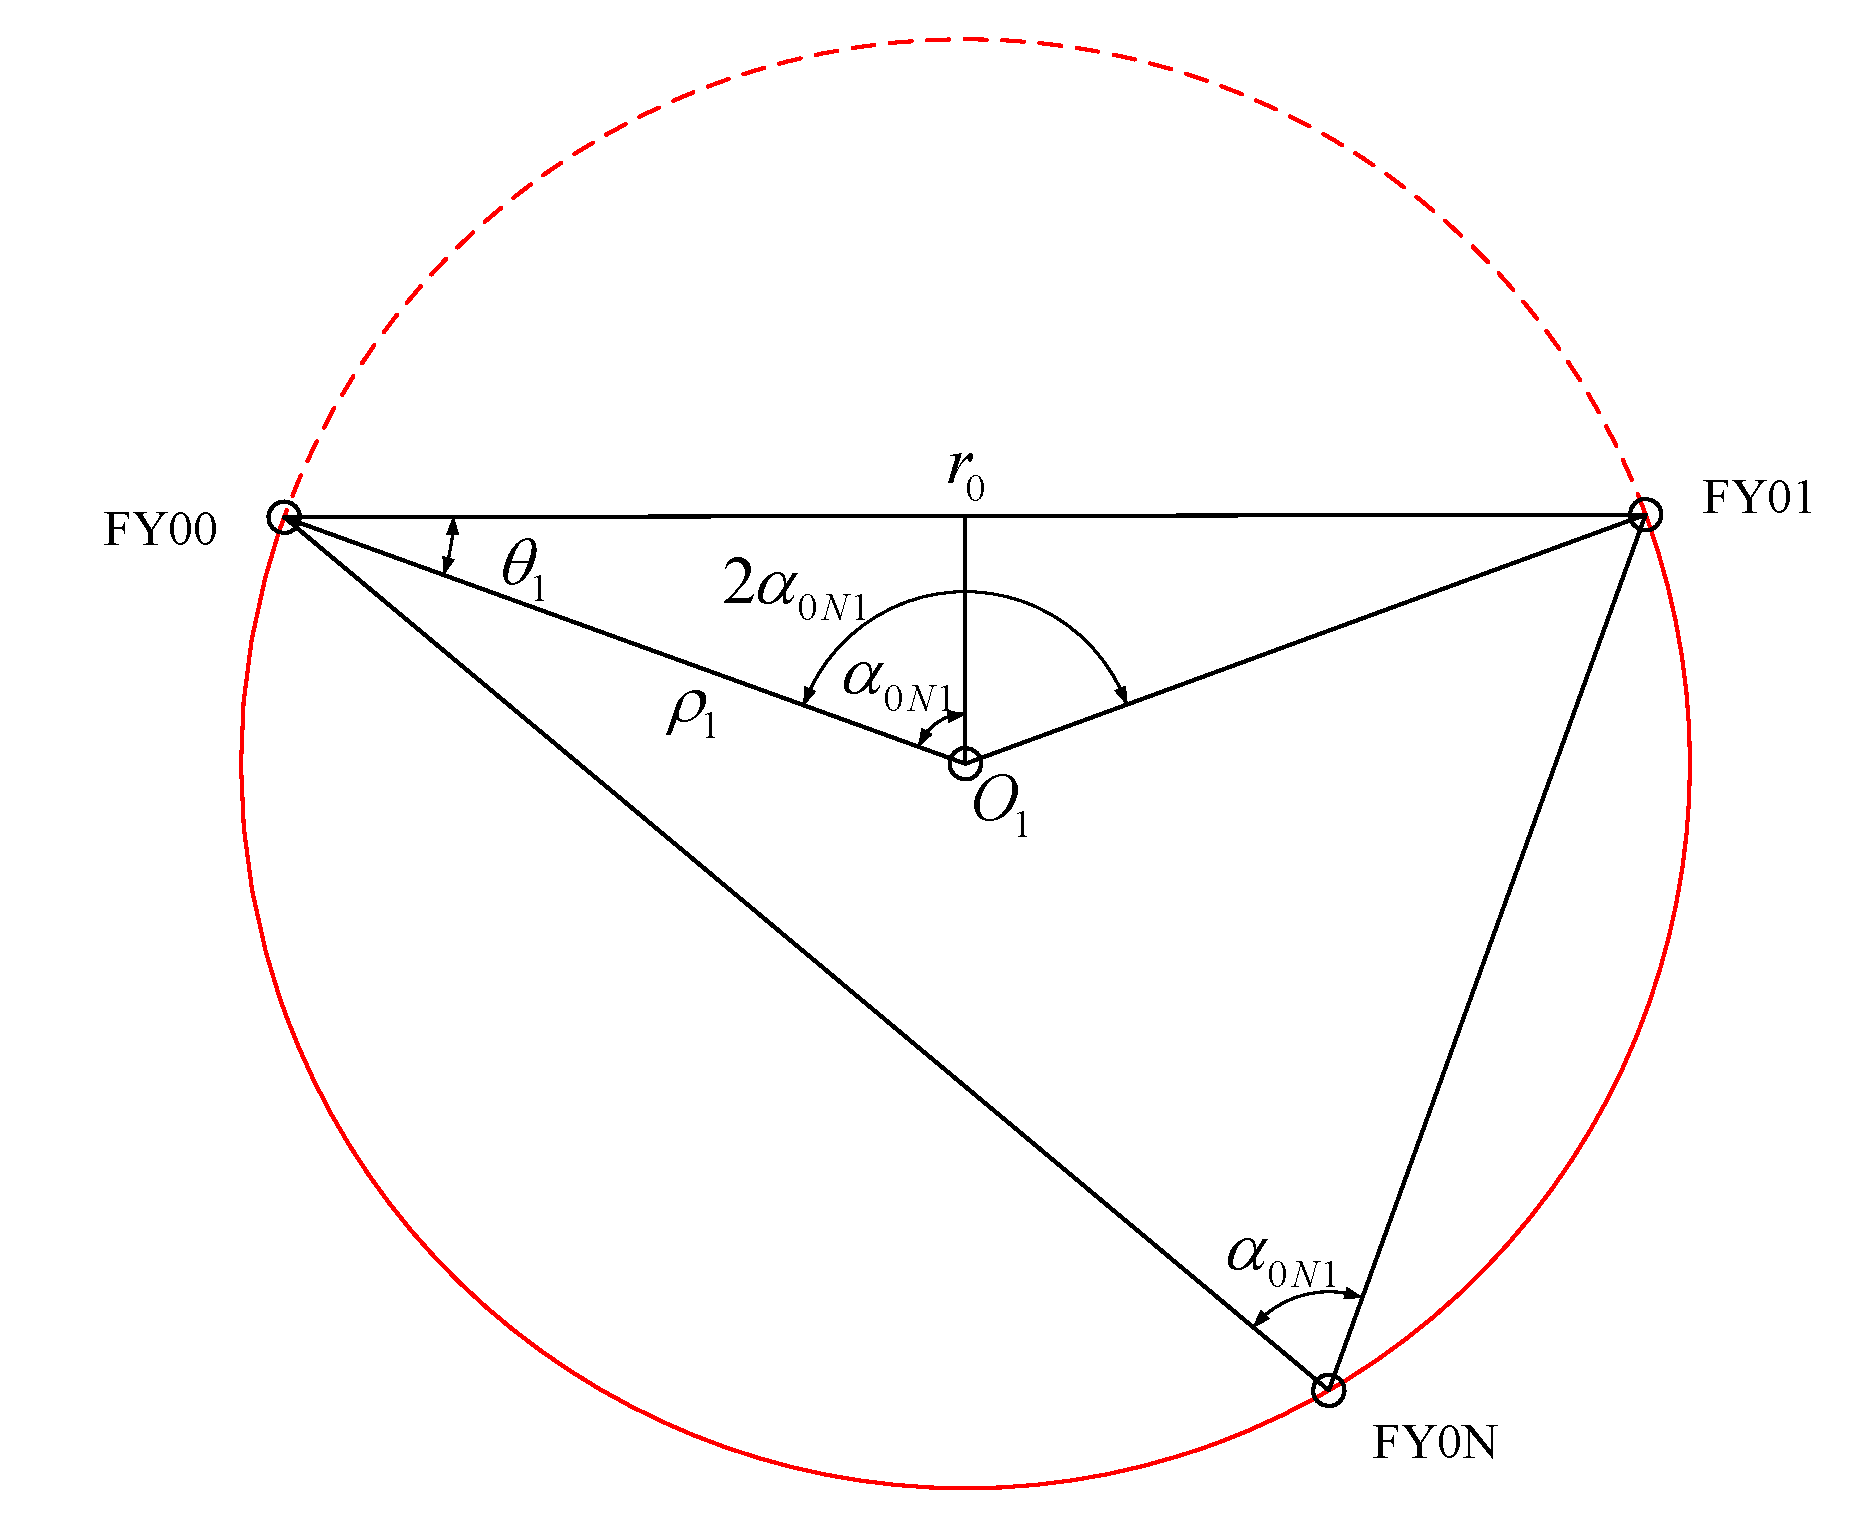
\includegraphics[width=\textwidth]{图片/问题1-1示意图 - 局部.pdf}
        \end{figure}
        \column{0.65\textwidth}
        我们以红色下半部分圆弧为例,来讨论圆心的坐标,如左图所示。从中我们可以得到,确定圆心坐标的两个重要的参数:
        \begin{align}
            \rho_1 &= \frac{r_0}{2\sin \alpha_{0N1}}\\
            \theta_1 &= \frac{\pi}{2} - \alpha_{0N1}
        \end{align}
        这样,我们可以得到$O_1$的极坐标为:
        \begin{equation}
            A = \left(\rho_1,-\theta_1\right) = \left(\frac{r_0}{2\sin \alpha_{0N1}}, - \frac{\pi}{2} + \alpha_{0N1}\right)
        \end{equation}
    \end{columns}
\end{frame}

\begin{frame}{基于两圆相交的定位模型}
    \begin{columns}
        \column{0.35\textwidth}
        \begin{figure}[!ht]
            \centering
            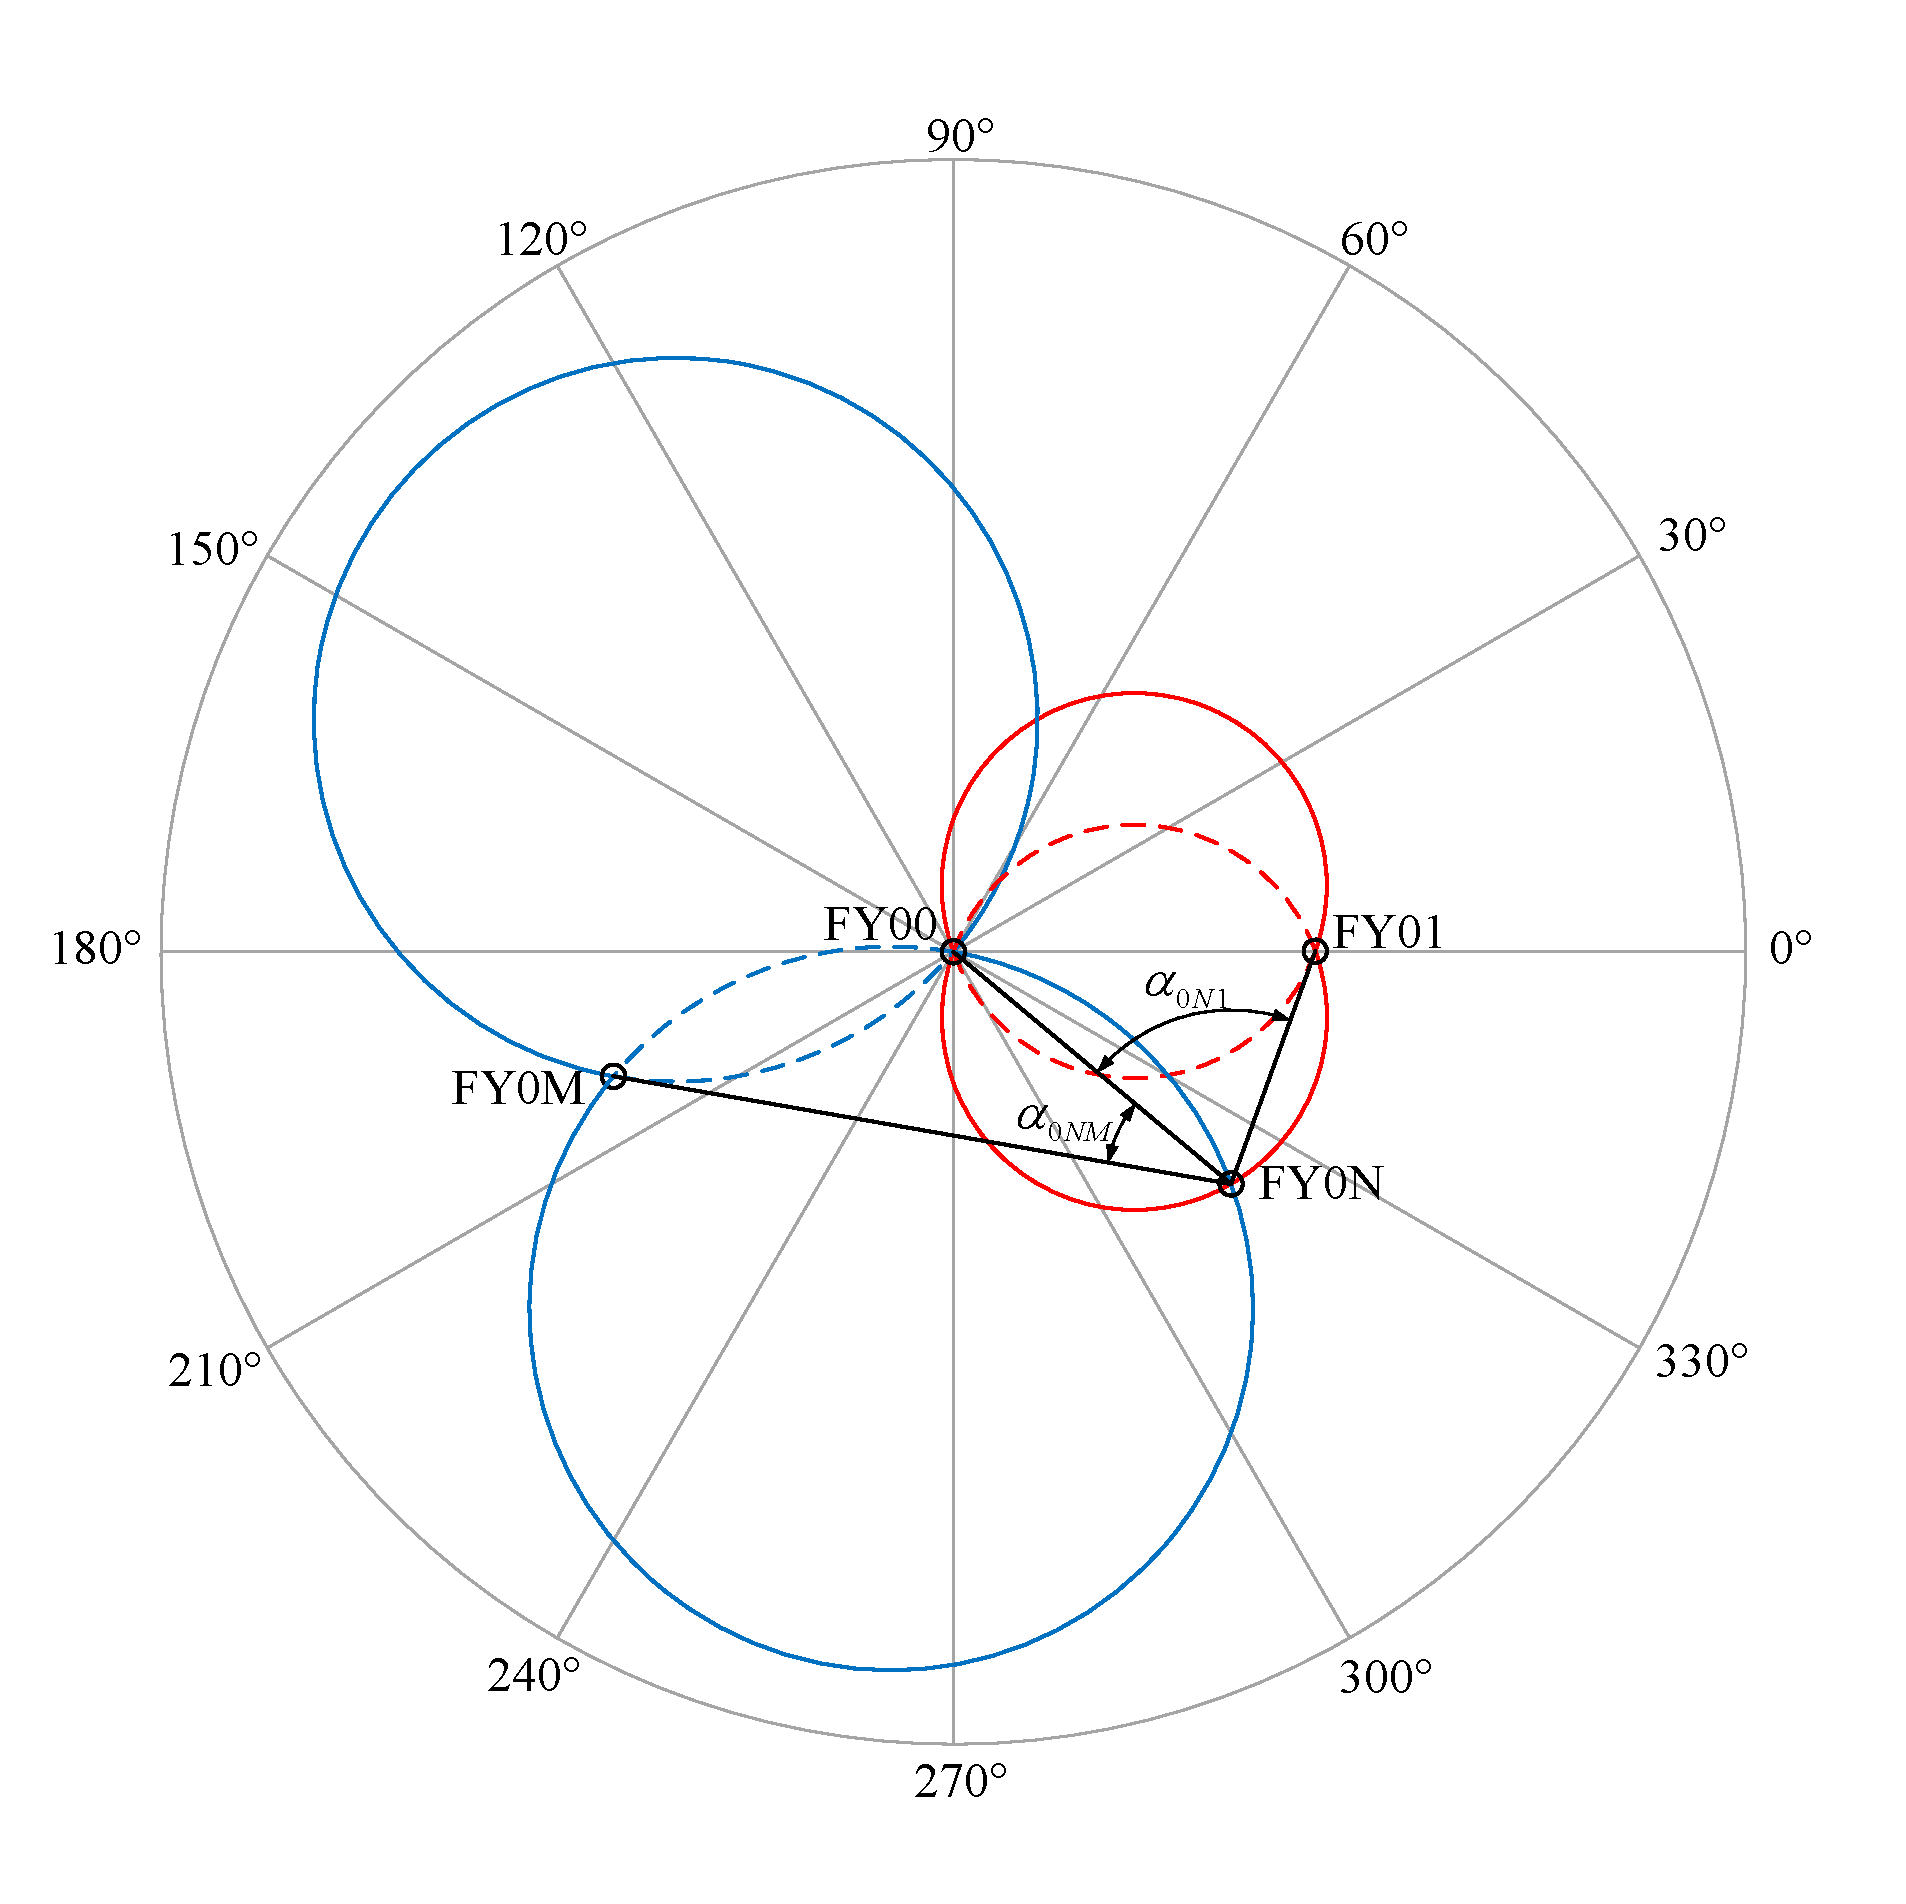
\includegraphics[width=\textwidth]{图片/问题1-1示意图.pdf}
        \end{figure}
        \column{0.65\textwidth}
        同理,我们可以得到与其对应的圆的圆心坐标,以及蓝色圆弧的圆心坐标。设FY00,FY01和FY0N组成的圆的圆心坐标为$A_{0N1}$,FY00,FY0M和FY0N组成的圆的圆心坐标为$A_{0NM}$,则其可以表示为:
        \begin{align}
            A_{0N1} &= \left(\frac{r_0}{2\sin \alpha_{0N1}}, 0 \pm \left(\frac{\pi}{2} - \alpha_{0N1}\right)\right)\\
            A_{0NM} &= \left(\frac{r_0}{2\sin \alpha_{0NM}}, \frac{2}{9}\left(m-1\right)\pi \pm \left(\frac{\pi}{2} - \alpha_{0NM}\right)\right)\label{eq:0NM圆心坐标}
        \end{align}
    \end{columns}
\end{frame}

\begin{frame}{基于两圆相交的定位模型}
    我们知道,极坐标下,圆心在$(\rho_0,\theta_0)$,半径为$r_0$的圆的一般方程为:
    \begin{equation}
        \rho^2 + \rho_0^2 - 2\rho\,\rho_0\cos\left(\theta - \theta_0\right) = r_0^2
    \end{equation}
    我们将两个圆的信息带入,可以得到如下方程组:
    \begin{equation}
        \left\{
        \begin{aligned}
            \rho^2 + \rho_{0N1}^2 - 2\rho\,\rho_{0N1}\cos\left(\theta - \theta_{0N1}\right) &= \rho_{0N1}^2\\
            \rho^2 + \rho_{0NM}^2 - 2\rho\,\rho_{0NM}\cos\left(\theta - \theta_{0NM}\right) &= \rho_{0NM}^2
        \end{aligned}
        \right.
    \end{equation}
    显然原点是一个解,我们不考虑原点情况,那么可以将$\rho$约去,得到:
    \begin{equation}
        \left\{
        \begin{aligned}
            \rho &= \frac{r_0}{\sin \alpha_{0N1}}\left(\cos\theta\,\cos\theta_{0N1} + \sin\theta\,\sin\theta_{0N1}\right)\\
            \rho &= \frac{r_0}{\sin \alpha_{0NM}}\left(\cos\theta\,\cos\theta_{0NM} + \sin\theta\,\sin\theta_{0NM}\right)
        \end{aligned}
        \right.
    \end{equation}
\end{frame}

\begin{frame}{基于两圆相交的定位模型}
    整理可以得到:
    \begin{equation}
        \cos\theta\frac{\cos\theta_{0N1}}{\sin\alpha_{0N1}} - \cos\theta\frac{\cos\theta_{0NM}}{\sin\alpha_{0NM}} =
        \sin\theta\frac{\sin\theta_{0NM}}{\sin\alpha_{0NM}} - \sin\theta\frac{\sin\theta_{0N1}}{\sin\alpha_{0N1}}
    \end{equation}

    进一步化简可以得到:
    \begin{equation}
        \tan\theta = \frac
        {\frac{\cos\theta_{0N1}}{\sin\alpha_{0N1}} - \frac{\cos\theta_{0NM}}{\sin\alpha_{0NM}}}
        {\frac{\sin\theta_{0NM}}{\sin\alpha_{0NM}} - \frac{\sin\theta_{0N1}}{\sin\alpha_{0N1}}}
    \end{equation}

    最终我们得到了$\tan\theta$的表达式,由假设可知,正常情况下,不会出现$\tan\theta$无意义的情况(这要求FY03和FY08的极角偏移为$\frac{1}{18}\pi$)。求出$\theta$后,我们可以得到:
    \begin{equation}
        \rho = \frac{r_0}{\sin \alpha_{0N1}}\left(\cos\theta\,\cos\theta_{0N1} + \sin\theta\,\sin\theta_{0N1}\right)
        \label{eq:极径计算}
    \end{equation}
\end{frame}

\begin{frame}{基于两圆相交的定位模型}
    但是接下来,我们依然有两个问题需要解决:
    \begin{itemize}
        \item $\theta_{0N1}$和$\theta_{0NM}$的取值有两个,我们需要确定选择哪一个;
        \item 在$0$到$2\pi$范围内,有两个$\theta$的取值使得$\tan\theta$为某一特定值,我们需要确定选择哪一个。
    \end{itemize}
\end{frame}

\subsection{特定情况下的讨论}

\begin{frame}{$\theta_{0N1}$和$\theta_{0NM}$值的确定}
    \begin{columns}
        \column{0.4\textwidth}
        \begin{figure}[!ht]
            \centering
            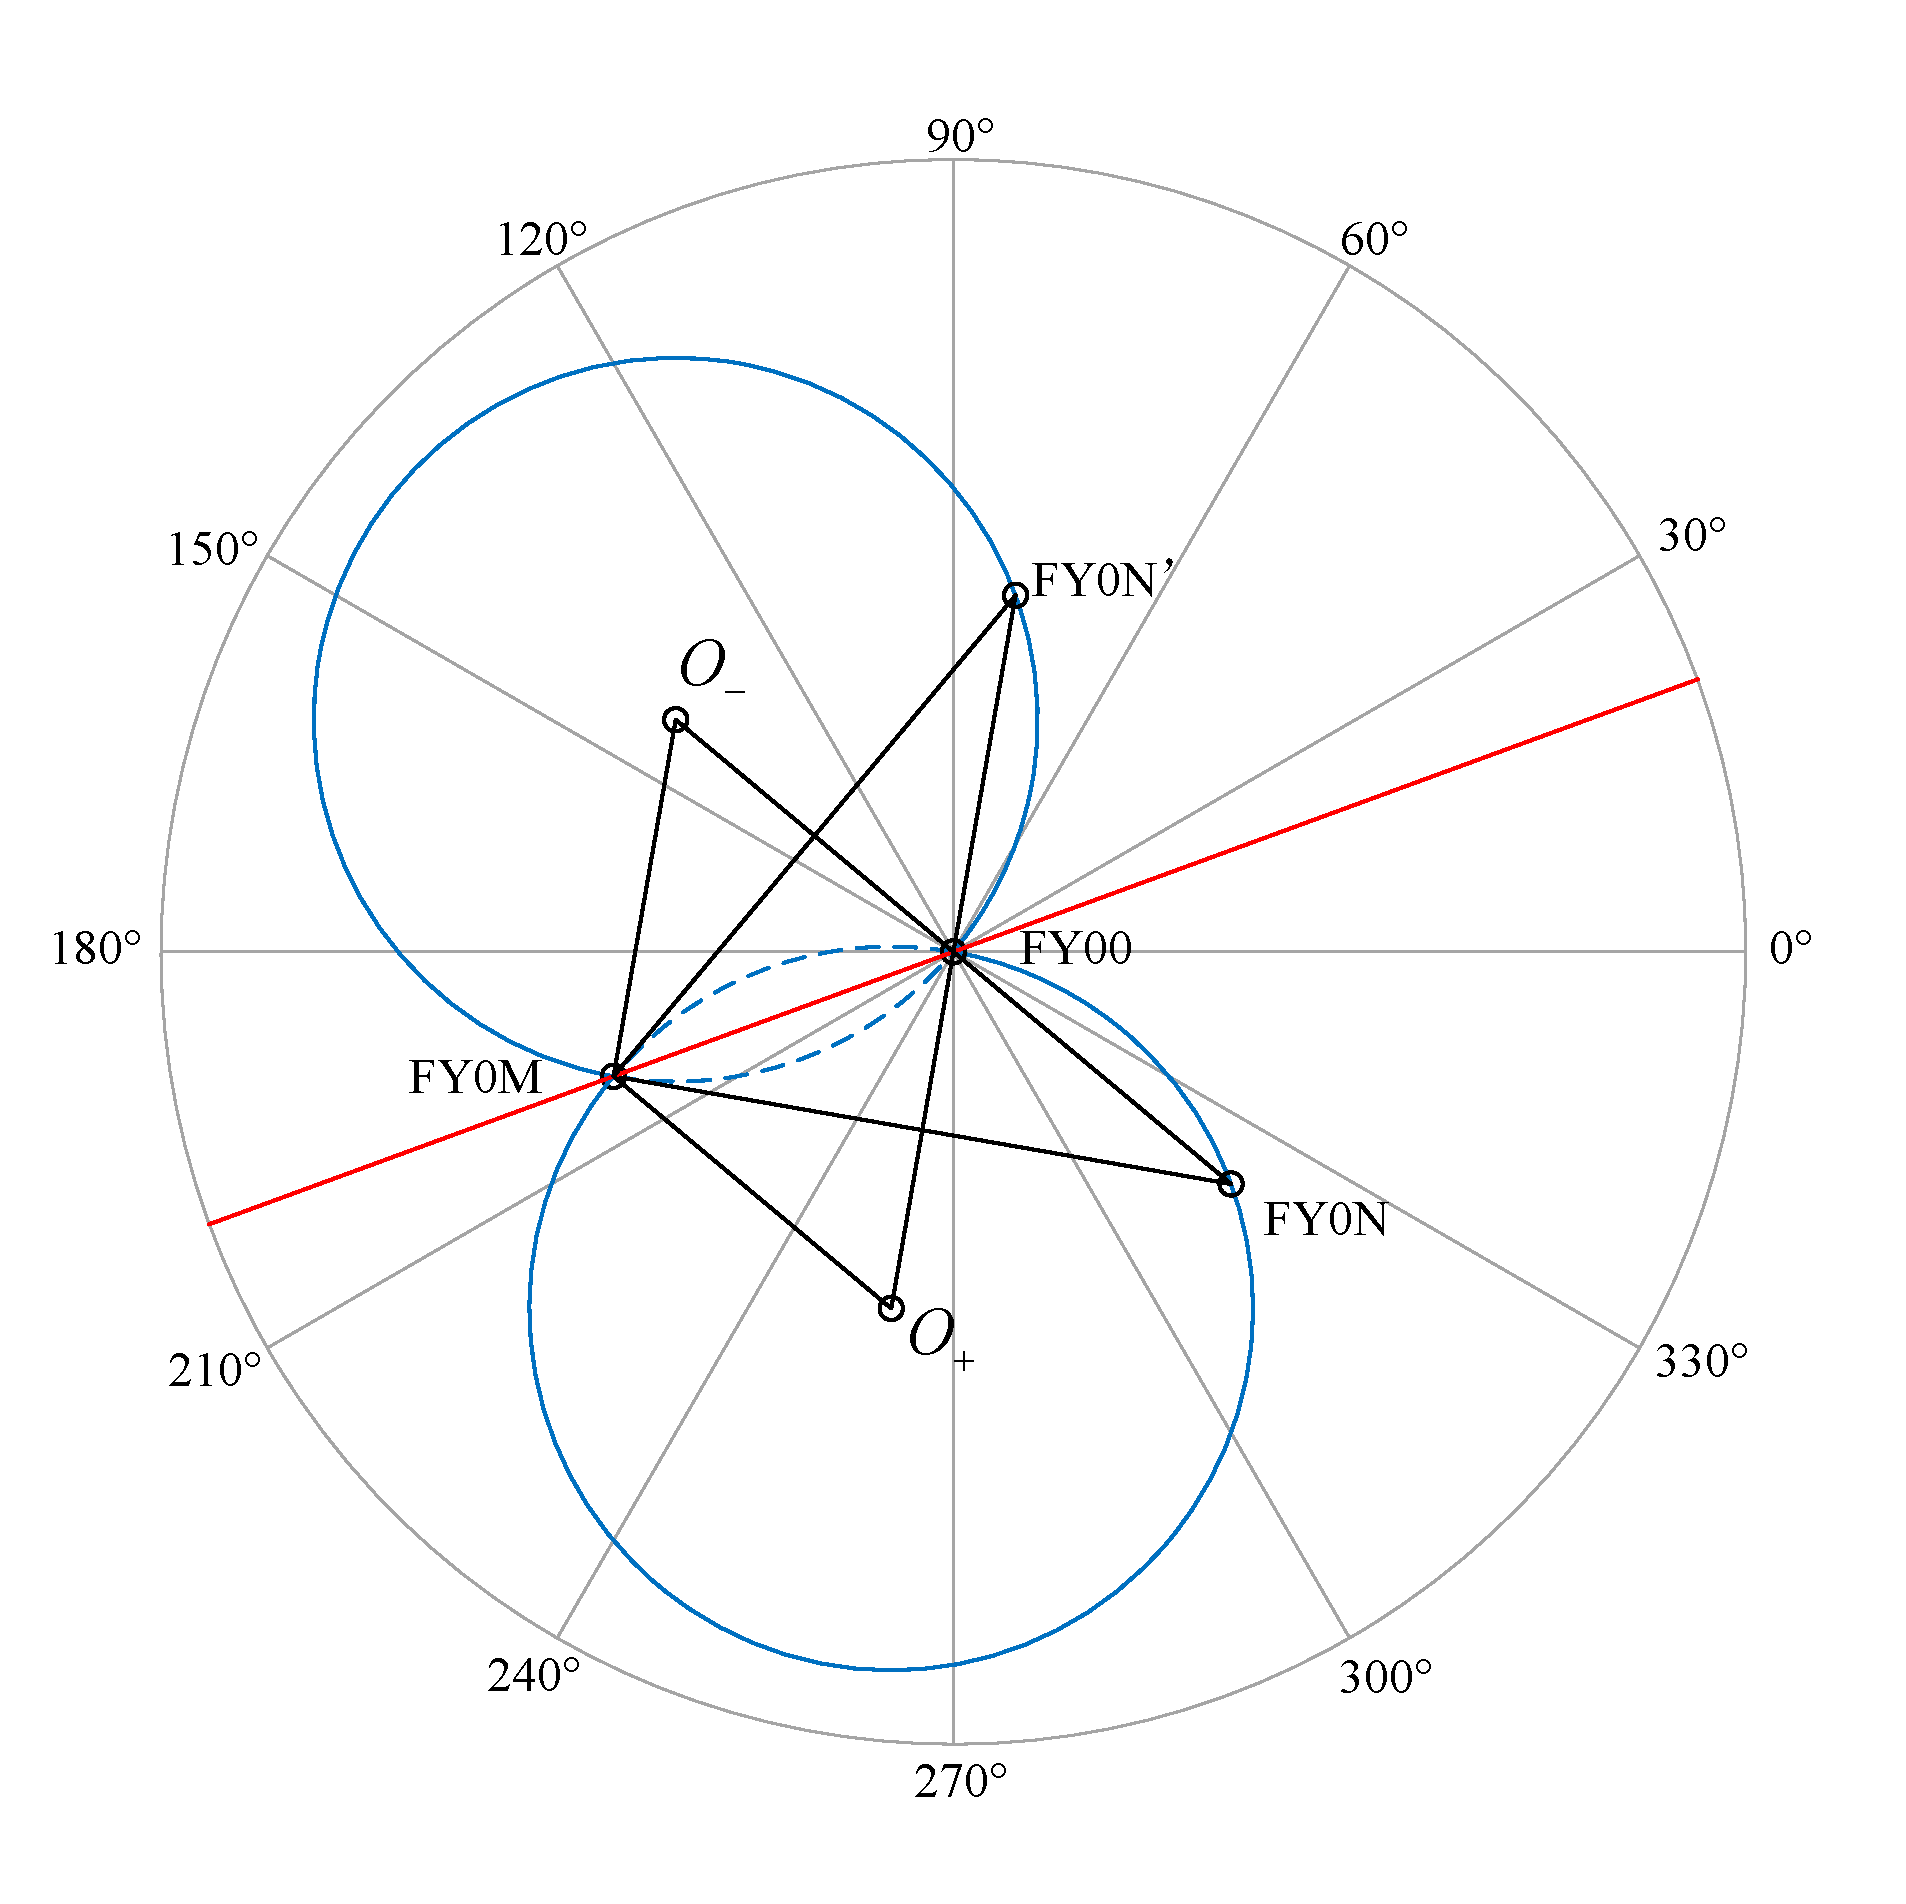
\includegraphics[width=\textwidth]{图片/theta取值讨论.pdf}
        \end{figure}
        \column{0.6\textwidth}
        现在我们观察左图。我们从中可以看到,对于$\theta_{0NM}$来说,$\frac{2}{9}\left(m-1\right)\pi \pm \left(\frac{\pi}{2} - \alpha_{0NM}\right)$中取$+$还是$-$,取决于,FY0N位于FY0M和FY00连成的直线(左中红色直线)的上方或者是下方(当正好位于直线上时,外接圆不存在)。
    \end{columns}
\end{frame}

\begin{frame}{$\theta_{0N1}$和$\theta_{0NM}$值的确定}
    设FY0N在极坐标系下的极角为$\theta_n$用数学语言表达就是:
        \begin{equation}
            \theta_{0NM} = \left\{
            \begin{aligned}
                & \frac{2}{9}\left(m-1\right)\pi + \left(\frac{\pi}{2} - \alpha_{0NM}\right)&&,
                0 < \theta_n - \frac{2}{9}\left(m-1\right)\pi + 2k\pi< \pi\\
                & \frac{2}{9}(m-1)\pi - \left(\frac{\pi}{2} - \alpha_{0NM}\right)&&,
                \pi < \theta_n - \frac{2}{9}(m-1)\pi + 2k\pi < 2\pi
            \end{aligned}
            \right.
        \end{equation}
        其中,$k \in \mathbb{Z}$。
        在假设前提下,略有偏差的位置不会影响FY0N与直线的位置关系,那么我们就可以得到:
        \begin{equation}
            \theta_{0NM} = \left\{
            \begin{aligned}
                & \frac{2}{9}\left(m-1\right)\pi + \left(\frac{\pi}{2} - \alpha_{0NM}\right)&&,
                0 < n - m + 9k < \frac{9}{2}\\
                & \frac{2}{9}\left(m-1\right)\pi - \left(\frac{\pi}{2} - \alpha_{0NM}\right)&&,
                \frac{9}{2} < n - m + 9k < 9
            \end{aligned}
            \right.
        \end{equation}
\end{frame}

\begin{frame}{$\theta_{0N1}$和$\theta_{0NM}$值的确定}
    同理,我们可以得到$\theta_{0N1}$在不同情况下的取值。下表展示了对于不同的$n$和$m$,$\theta_{0N1}$和$\theta_{0NM}$的取值。
    \begin{table}[!ht]
        \centering
        \footnotesize
        \begin{tabular}{ccc}
            \toprule
            ~  &  $1 \leq n - m + 9k \leq 4$ & $5 \leq n - m + 9k \leq 8$\\
            \midrule
            $2 \leq n \leq 5$ & 
            $
            \left\{
            \begin{aligned}
                \theta_{0N1} &= \frac{\pi}{2} - \alpha_{0N1}\\
                \theta_{0NM} &= \frac{2}{9}\left(m-1\right)\pi + \left(\frac{\pi}{2} - \alpha_{0NM}\right)
            \end{aligned}
            \right.
            $
            & 
            $
            \left\{
            \begin{aligned}
                \theta_{0N1} &= \frac{\pi}{2} - \alpha_{0N1}\\
                \theta_{0NM} &= \frac{2}{9}\left(m-1\right)\pi - \left(\frac{\pi}{2} - \alpha_{0NM}\right)
            \end{aligned}
            \right.
            $
            \\
            $6 \leq n \leq 9$ &
            $
            \left\{
            \begin{aligned}
                \theta_{0N1} &= - \frac{\pi}{2} + \alpha_{0N1}\\
                \theta_{0NM} &= \frac{2}{9}\left(m-1\right)\pi + \left(\frac{\pi}{2} - \alpha_{0NM}\right)
            \end{aligned}
            \right.
            $
            & 
            $
            \left\{
            \begin{aligned}
                \theta_{0N1} &= - \frac{\pi}{2} + \alpha_{0N1}\\
                \theta_{0NM} &= \frac{2}{9}\left(m-1\right)\pi - \left(\frac{\pi}{2} - \alpha_{0NM}\right)
            \end{aligned}
            \right.
            $
            \\
            \bottomrule
        \end{tabular}
    \end{table}
\end{frame}

\begin{frame}{$\theta$值的确定}
    我们不能直接使用$\arctan\tan\theta$来作为$\theta$的值,因为$\arctan$函数的值域是$\left(-\frac{\pi}{2},\frac{\pi}{2}\right)$,而我们需要的$\theta$的值域是$\left(0,2\pi\right)$。在无人机的位置仅仅略有偏差(这里要求极角偏差小于$\frac{1}{18}\pi$,否则会出现跨区域问题)的情况下,我们可以通过$n$的取值,来判断$\theta$的取值范围,然后再通过$\tan\theta$的值来确定$\theta$的具体取值。如下表所示。
    \begin{table}[!ht]
        \centering
        \begin{tabular}{cc}
            \toprule
            ~  &  $\theta$\\
            \midrule
            $n=2,3$ & $\arctan\tan\theta$\\
            $n=4,5,6,7$ & $\arctan\tan\theta + \pi$\\
            $n=8,9$ & $\arctan\tan\theta + 2\pi$\\
            \bottomrule
        \end{tabular}
    \end{table}
\end{frame}

%%%%%%%%%%%%%%%%%%%%%%%%%%%%%%%%%%%%%%%%%%%%%%%%%%%%%%%%%%%%%%%%
%                                                              %
%%%%%%%%%%%%%%%%%%%%%%%%%%%%%%%%%%%%%%%%%%%%%%%%%%%%%%%%%%%%%%%%

\section[问题1-2]{问题一(2)无人机有效定位条件}

\subsection{通过角度信息估算发射信号无人机序数}

\begin{frame}{通过角度信息估算发射信号无人机序数}
    \begin{columns}
        \column{0.4\textwidth}
        \begin{figure}[!ht]
            \centering
            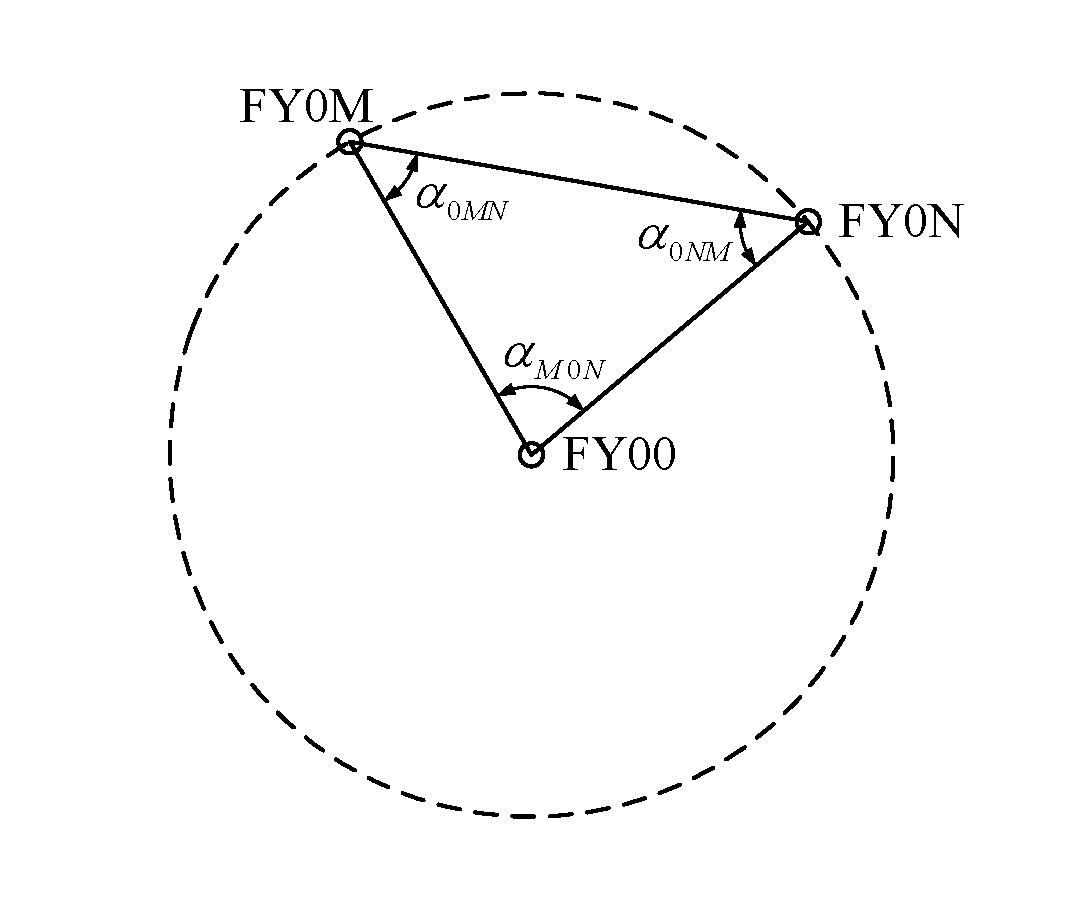
\includegraphics[width=\textwidth]{图片/问题1-2示意图1.pdf}
        \end{figure}

        \column{0.6\textwidth}
        对于任意两个无人机,假设其编号分别为$n$和$m$,则如左图所示。
        
        如果,FY0M和FY0N的位置是准确的,因为9架无人机均匀分布在圆周上,我们可以得到:
        \begin{equation}
            \alpha_{M0N} = \frac{2}{9}\pi\left|n-m\right|
        \end{equation}
    
        根据等腰三角形的性质,我们很容易可以得到:
        \begin{equation}
            \alpha_{0MN} = \alpha_{0NM} = \frac{1}{2}\pi - \frac{1}{9}\pi\left|n-m\right|
        \end{equation}
    \end{columns}
\end{frame}

\begin{frame}
    通过上面的式子,即使在FY0M和FY0N的位置略有偏差的情况下,我们也可以通过$\alpha_{0MN}$和$\alpha_{0NM}$的值,来估计$|n-m|$的值。我们以$\alpha_{0MN}$为例,我们可以得到:
    \begin{equation}
        \left|n-m\right| \approx 9\left(\frac{1}{2} - \frac{\alpha_{0MN}}{\pi}\right)
    \end{equation}

    为了使得对$\left|n-m\right|$的估计不出现错误,$\alpha_{0MN}$的误差应当小于$\frac{1}{18}\pi$,也就是:
    \begin{equation}
        \Delta\alpha_{0MN} < \frac{1}{18}\pi
        \label{eq:误差条件}
    \end{equation}
    接下来的讨论都将以此为基础。

    显然,对于一个$m$,有两个$n$的可能取值满足条件,分别记为$n_1$和$n_2$,为了简化后续叙述,我们称FY0N1与FY0N2关于FY0M对称。
\end{frame}

\subsection{额外一架无人机的情况}

\begin{frame}{额外一架无人机的情况}
    \begin{columns}
        \column{0.4\textwidth}
        \begin{figure}[!ht]
            \centering
            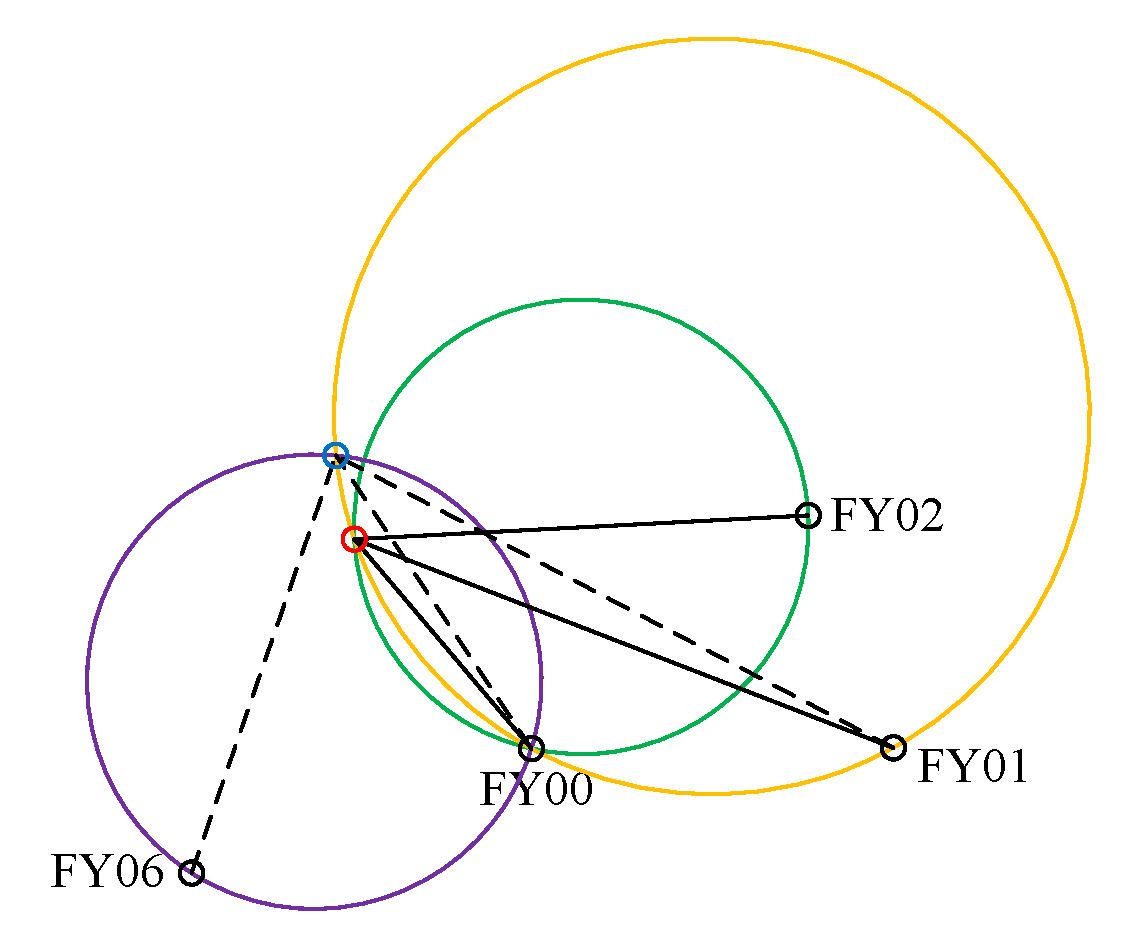
\includegraphics[width=\textwidth]{图片/问题1-2示意图2.pdf}
        \end{figure}

        \column{0.6\textwidth}
        现在我们来讨论,如左图所示的情况。FY04的位置略有偏差,其实际位置位于图中红色圆圈标识的位置。
        \begin{itemize}
            \item 通过FY01和FY00的信息,其知道自身在橙色圆周上;
            \item 通过来源未知(实际是FY02)的约为$\frac{7}{18}\pi$的角度信息,其估计发射信号源为FY02或者FY06;
            \item 其可以确定自己的位置在图中绿色圆周或者紫色圆周上。
        \end{itemize}
        但是FY04无法确定自身位置,有两个点符合上述的条件。所以只有额外一架无人机提供的角度信息是不够的。
    \end{columns}
\end{frame}

\begin{frame}{额外一架无人机的情况}
    为简便后续讨论,我们称因为对发射信号的无人机序数的误判而推导出的错误位置称为“幻觉”。

    这种这种位置的不确定性起始来自于发射信号的无人机的位置不缺定性。所以在以下两种情况下,接收信号的无人机可以确定自身的位置:
    \begin{itemize}
        \item 发射信号的无人机的位置确定。设FY0M接收信号,FY0N为FY0M不知道序号的信号发射者。如果FY0N和FY01关于FY0M对称,则FY0M可以确定自己的位置,因为FY01不可能向它发射两个信号。
        \item 发射信号的无人机的位置不确定性不影响定位。“幻觉”位置和真实位置相同,也就是两个可能点的位置重合。
    \end{itemize}
\end{frame}

\begin{frame}{额外一架无人机的情况}
    \begin{columns}
        \column{0.4\textwidth}
        \begin{figure}[!ht]
            \centering
            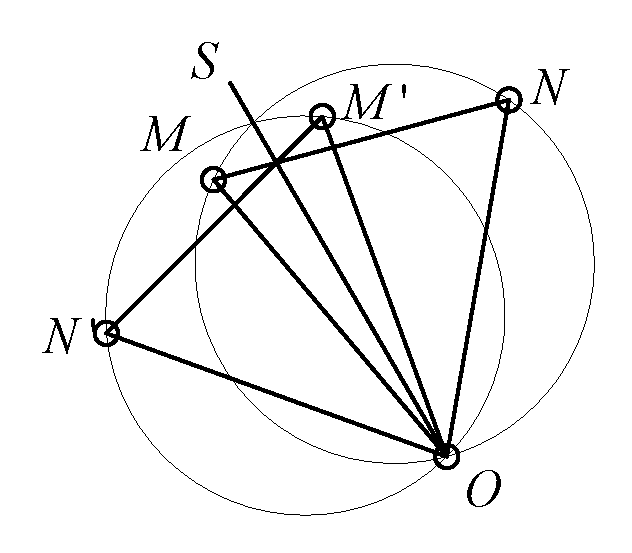
\includegraphics[width = \textwidth]{图片/幻觉重合.pdf}
        \end{figure}

        \column{0.6\textwidth}
        我们现在来讨论第二点。左图中,$O$为圆心无人机,$N$为发射信号的无人机,$N'$为可能被误认为是发射信号无人机的无人机。$M$为任意满足$\angle OMN$为接收到信号角度的点,$OS$为$\angle NON'$的角平分线,$M'$为$M$关于$OS$的对称点。

        由已有条件,我们可以得到:$OM=OM'$,$\angle MOS = \angle M'OS$,$\angle NOS = \angle N'OS$。我们可以得到:
        \begin{equation}
            \angle MON = \angle M'ON'
        \end{equation}
        则可以根据,全等三角形的边角边定理,得到$\bigtriangleup MON \cong \bigtriangleup M'ON'$。则可以得到:
        \begin{equation}
            \angle N'M'O = \angle NMO
        \end{equation}
    \end{columns}
\end{frame}

\begin{frame}{额外一架无人机的情况}
    这样构建起了一个到一一对应关系,对于一个点$M$,我们可以找到一个点$M'$,$\angle N'M'O = \angle NMO$。我们知道,使得$\angle NMO$为固定值的点,在经过$N$和$O$且半径固定的圆上。则使得$\angle N'M'O$为相同固定值的点,在其关于$OS$对称的圆上。

    这两个圆交与2点,一个是点$O$,另一个点在$OS$上。也就是说,只有点$M$在$OS$上时,才能满足$\angle OMN = \angle OMN'$。

    换言之,想要“幻觉”与真实位置相同,则需要满足$\angle OMN = \angle OMN'$。所以,其必须在$OS$上,如果$N$和$N'$的位置是准确的,那么等价于$M$在极坐标系的极角是与正确位置相同的。
\end{frame}

\subsection{额外两架无人机的情况}

\begin{frame}{额外两架无人机的情况}
    除了FY00和FY01外,还有序号分别为$m$和$n$的无人机FY0M和FY0N发射信号,序号为$p$的无人机FY0P接收信号,但是FY0P不知道除了FY00和FY01外的发射信号无人机的序号。序号为$p$的无人机接收到三个角度信息,分别为$\alpha_{0PM}$,$\alpha_{0PN}$和$\alpha_{0P1}$。和上面相同,除了正确位置外,$\alpha_{0PM}$,$\alpha_{0PN}$各会误导出一个错误的位置,我们称之为“幻觉”。只要两个“幻觉”的位置不同,FY0P就可以通过投票的方式得到自己的真实位置。
\end{frame}

\begin{frame}{额外两架无人机的情况}
    由上面的讨论我们可以知道,如果出现以下情况,FY0P可以确定自身位置:
    \begin{itemize}
        \item 如果,待确定位置无人机的位置的在极坐标系下的极角是正确的,则根据上面的讨论,两个幻觉都和正确位置重合,FY0P可以确定自己的位置。
        \item 如果,两个额外发射信号无人机中的任何一架,关于FY0P于与FY01对称,则FY0P可以立即确定自身位置。
    \end{itemize}
\end{frame}

\begin{frame}{额外两架无人机的情况}
    \begin{columns}
        \column{0.4\textwidth}
        \begin{figure}[!ht]
            \centering
            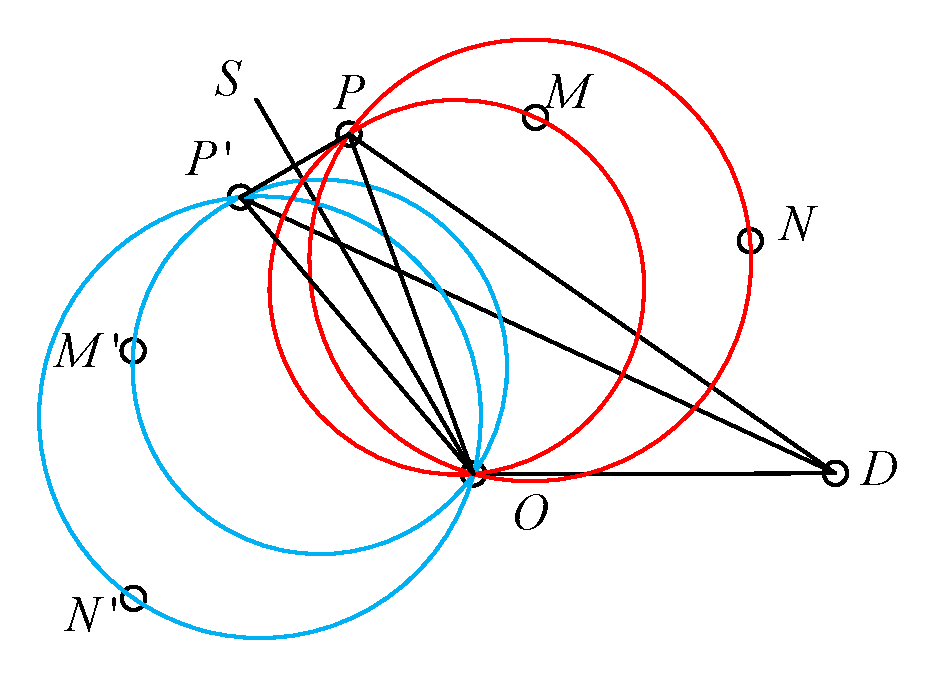
\includegraphics[width = \textwidth]{图片/两架无人机情况.pdf}
        \end{figure}

        \column{0.6\textwidth}
        接下来我们讨论一般情况。假设两个“幻觉”重合。如左图所示,图中$D$是FY01位置,$P$是真实位置,$M$和$N$为实际发射信号无人机位置,$M'$和$N'$为被误认为是发射信号无人机位置,$P'$为两个“幻觉重合的位置”。

        我们不讨论$P'$和$P$在$OD$两侧的情况,因为这至少要求FY05或FY06的极角偏差$\frac{1}{9}\pi$。
    \end{columns}
\end{frame}

\begin{frame}{额外两架无人机的情况}
    \begin{columns}
        \column{0.4\textwidth}
        \begin{figure}[!ht]
            \centering
            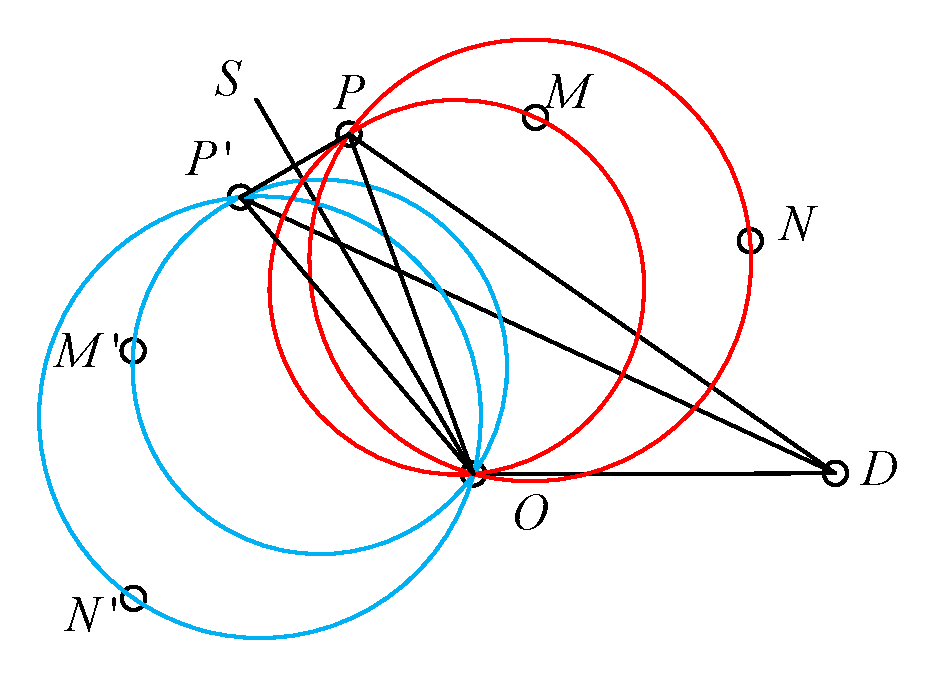
\includegraphics[width = \textwidth]{图片/两架无人机情况.pdf}
        \end{figure}

        \column{0.6\textwidth}
        因为$P$和$P'$关于$OS$对称:
        \begin{equation}
            OP = OP'
        \end{equation}
        然后,无论“幻觉”还是真实位置,都有:
        \begin{equation}
            \angle OPD = \angle OP'D
        \end{equation}
        那么$P'$和$P$在$OD$同侧,$O$、$D$、$P$、$P'$四点共圆。无论$D$在哪一侧,我们都可以得到:
        \begin{equation}
            \angle PDO + \angle PP'O = \pi
        \end{equation}
        由于$\bigtriangleup POP'$是等边三角形,$\angle PP'O$是锐角,这要求$\angle PDO$是钝角,
    \end{columns}
\end{frame}

\begin{frame}{额外两架无人机的情况}
    \begin{columns}
        \column{0.4\textwidth}
        \begin{figure}[!ht]
            \centering
            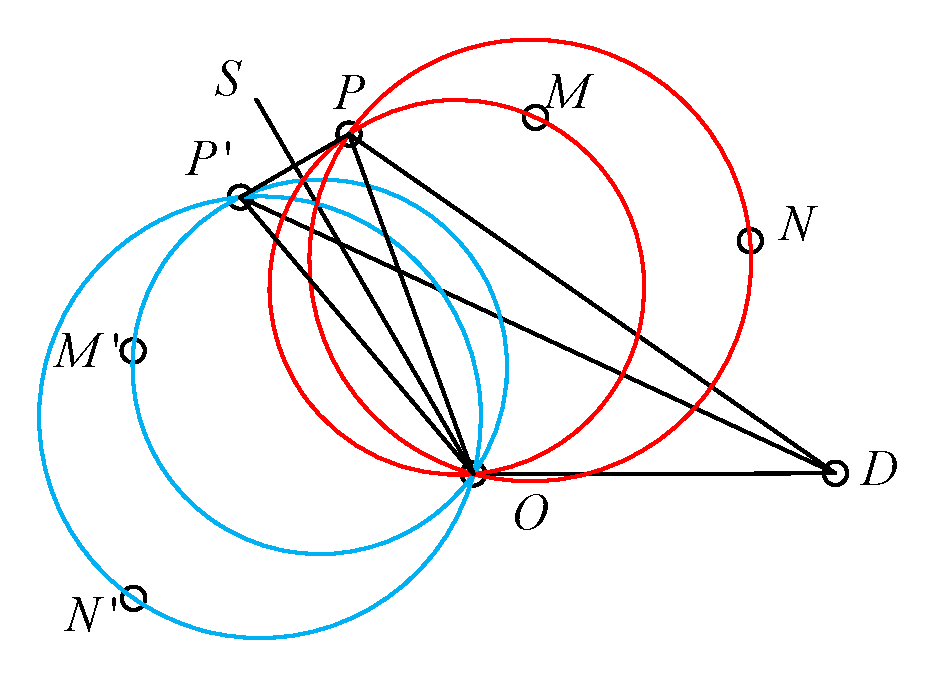
\includegraphics[width = \textwidth]{图片/两架无人机情况.pdf}
        \end{figure}

        \column{0.6\textwidth}
        若$\angle PDO$不是钝角,则假设不成立,两个“幻觉”不会重合于真实位置以外的点。

        对于FY02和FY09这两个靠近FY01的无人机来说,这个要求虽然苛刻,但是还是容易达到的。为了研究这一问题,我们以FY09为例,我们设$\Delta\theta$为FY09的极坐标偏差,$\Delta\rho$为FY09的极径偏差,满足以下关系时,$\angle PDO$是锐角:
        \begin{equation}
            \frac{\Delta\rho}{r_0} < \frac{1}{\cos\left(\frac{2\pi}{9}-\Delta\theta\right)} - 1
        \end{equation}
    \end{columns}
\end{frame}

\begin{frame}{额外两架无人机的情况}
    \begin{columns}
        \column{0.4\textwidth}
        \begin{figure}[!ht]
            \centering
            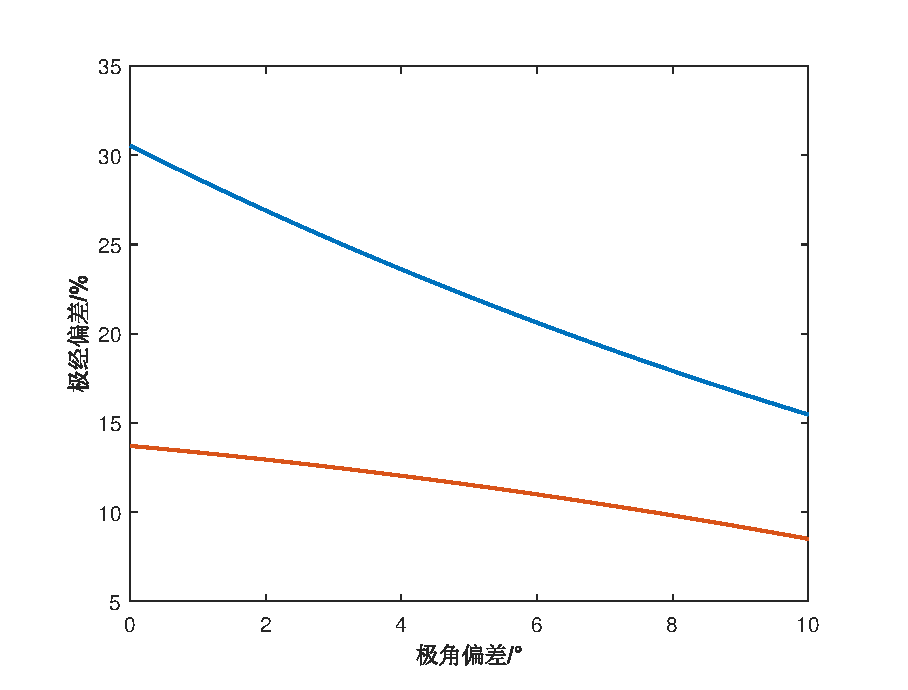
\includegraphics[width = \textwidth]{图片/极角极径偏差.eps}
        \end{figure}

        \column{0.6\textwidth}
        我们绘制了FY09在临界状态下,极角偏差与极径偏差的关系图,如左图中蓝色曲线所示,高于曲线的部分,可能会产生FY0P无法确定自身位置的情况。图中橙色曲线,则为式\ref{eq:误差条件}的要求,高于曲线的部分,FY0P会无法确定发射信号的无人机。\ref{eq:误差条件}的要求完全覆盖了$\angle PDO$是锐角的要求。
        
        所以我们不需要引入额外的假设,就可以断言,在满足\ref{eq:误差条件}时,两架额外的无人机的角度信息足够确定FY0P的位置。
    \end{columns}
\end{frame}


%%%%%%%%%%%%%%%%%%%%%%%%%%%%%%%%%%%%%%%%%%%%%%%%%%%%%%%%%%%%%%%%
%                                                              %
%%%%%%%%%%%%%%%%%%%%%%%%%%%%%%%%%%%%%%%%%%%%%%%%%%%%%%%%%%%%%%%%

\section[问题1-3]{问题一(3)无人机编队调整}

\subsection{在角度指引下的无人机移动}

\begin{frame}{在角度指引下的无人机移动}
    如下图所示。$O$为在圆心的发射信号的无人机,$L_1$和$L_2$为在圆周上的两架发射信号的无人机,$R$为需要通过接收的信号调整位置的无人机。在这个例子中,$R$需要从$R_1$的位置移动到$R_2$的位置。
    \begin{figure}[!ht]
        \centering
        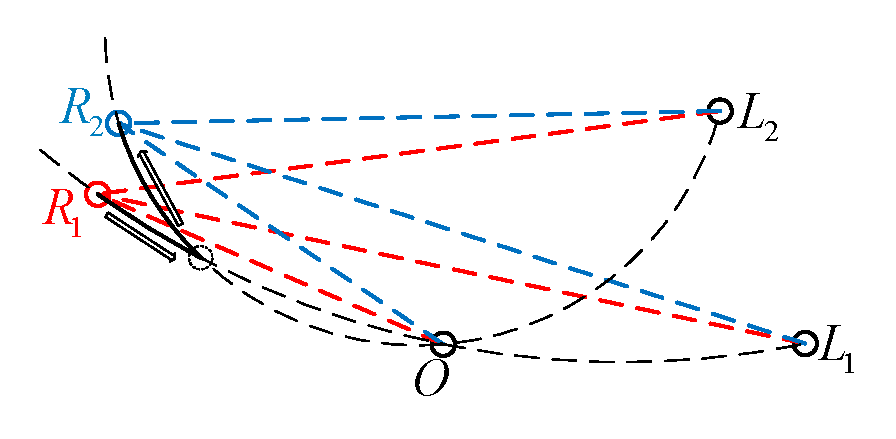
\includegraphics[width=0.6\textwidth]{图片/问题1-3示意图1.pdf}
    \end{figure}
\end{frame}

\begin{frame}{在角度指引下的无人机移动}
    我们给出如下的调整策略:
    \begin{enumerate}
        \item 保持$\angle ORL_1$不变为$\angle OR_1L_1$,顺着梯度方向或梯度下降方向,将$\angle ORL_2$从$\angle OR_1L_2$调整至$\angle OR_2L_2$;
        \item 保持$\angle ORL_2$不变为$\angle OR_2L_2$,顺着梯度方向或梯度下降方向,将$\angle ORL_1$从$\angle OR_1L_1$调整至$\angle OR_2L_1$。
    \end{enumerate}
    \begin{figure}[!ht]
        \centering
        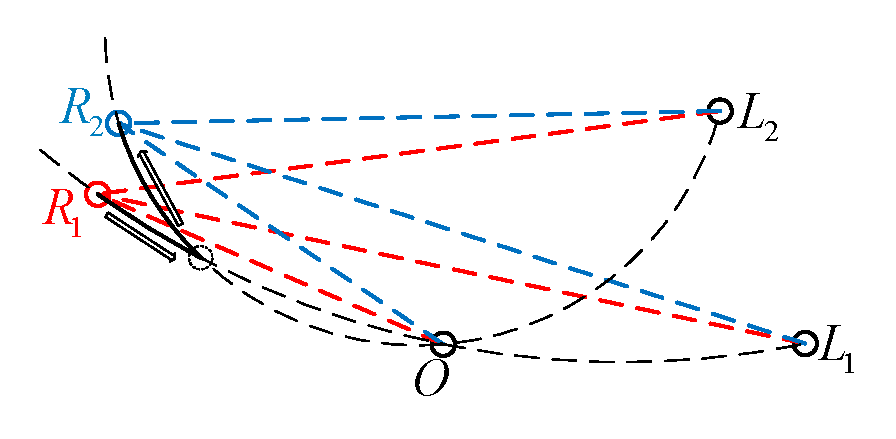
\includegraphics[width=0.5\textwidth]{图片/问题1-3示意图1.pdf}
    \end{figure}
\end{frame}

\begin{frame}{在角度指引下的无人机移动}
    调整的路线如下图中黑色实线和箭头所示。通过这种基于角度指引的无人机移动方案,通过一架位于圆心和两架位于圆周上的无人机发射信号,可以将一架接收信号的无人机在小范围内进行调整,使得其接收到的两个角度信息为指定值。
    \begin{figure}[!ht]
        \centering
        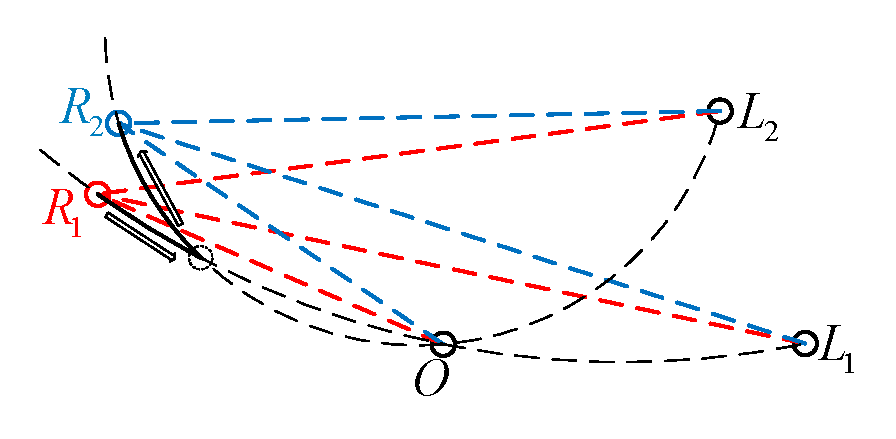
\includegraphics[width=0.6\textwidth]{图片/问题1-3示意图1.pdf}
    \end{figure}
\end{frame}

\subsection{无人机编队调整方案}

\begin{frame}{调整方案层次结构}
    我们的无人机调整有如下层次结构:
    \begin{itemize}
        \item 针对单架无人机进行单一目的的调整称为“步”;
        \item 所有无人机(除“半径标定机”外)都进行了一“步”调整则称为“轮”。
    \end{itemize}
\end{frame}

\begin{frame}{调整方案层次结构}
    我们的无人机调整方案共有两种“步”的调整方案:“角度矫正步”、“半径矫正步”。其原则如下:
    \begin{itemize}
        \item 角度矫正步:无人机接收两侧无人机和圆心无人机发出的信号。调整自身位置,使得自身接收到的角度信号为理想角度;
        \item 半径矫正步:无人机接收来关于“半径标定机”对称的无人机、“半径标定机”还有圆心无人机的信号,假设发射信号和接收信号的无人机角度信息是正确的。维持自身、FY00与“半径标定机”形成的夹角不变,调整自身位置,使自身距离FY00的距离与“半径标定机”距离FY00的距离相等。
    \end{itemize}
\end{frame}

\begin{frame}{角度矫正步}
    \begin{columns}
        \column{0.4\textwidth}
        \begin{figure}[!ht]
            \centering
            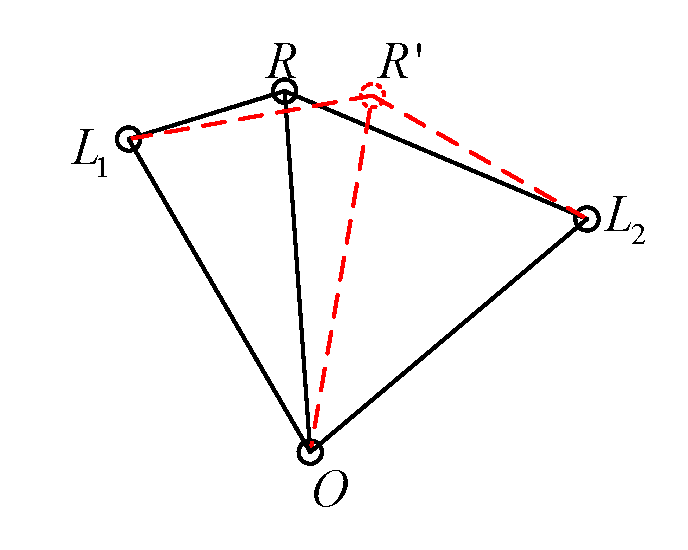
\includegraphics[width = \textwidth]{图片/角度矫正步.pdf}
        \end{figure}

        \column{0.6\textwidth}
        角度矫正步的调整方案:设任意一个无人机FY0N,其顺时针方向的下一个无人机为FY0N-1,逆时针方向的下一个无人机为FY0N+1。FY0N接收到的角度信息为$\alpha_{0NN-1}$和$\alpha_{0NN+1}$,我们需要调整其至$\alpha_{0NN-1}'$和$\alpha_{0NN+1}'$满足如下条件:
        \begin{equation}
            \alpha_{0NN-1}' = \alpha_{0NN+1}' = \frac{7}{18}\pi
        \end{equation}
    \end{columns}
\end{frame}

\begin{frame}{半径矫正步}
    半径矫正步设计如下两种情况:
    \begin{figure}[!ht]
        \centering
        \begin{minipage}[t]{0.2\textwidth}
            \centering
            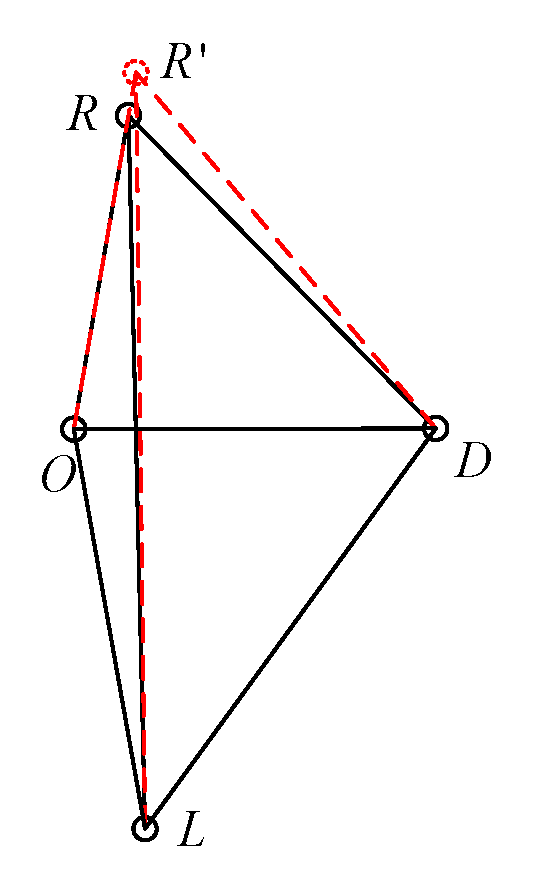
\includegraphics[width=\textwidth]{图片/半径矫正步1.pdf}
        \end{minipage}
        \hspace{0.1\textwidth}
        \begin{minipage}[t]{0.3\textwidth}
            \centering
            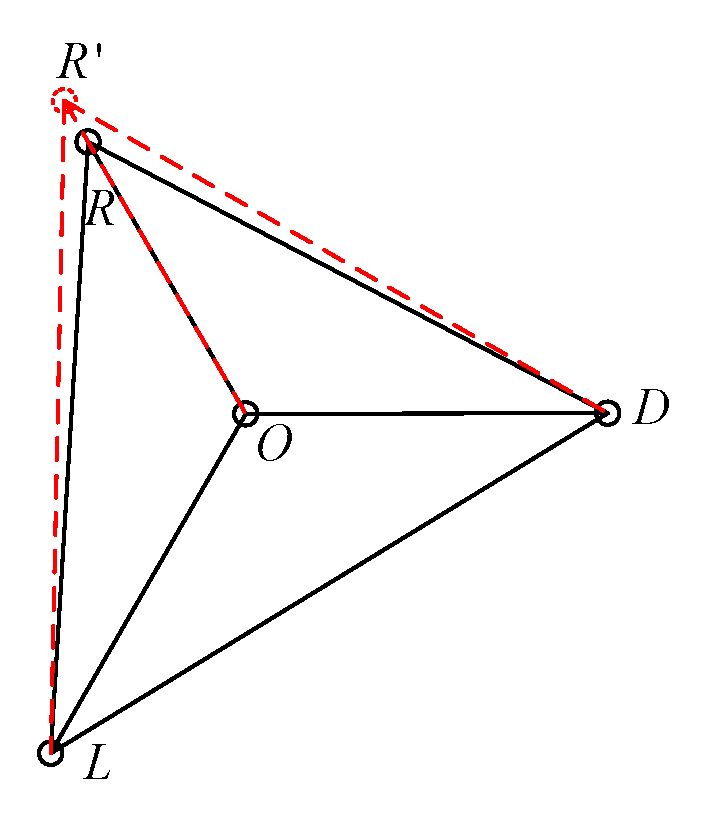
\includegraphics[width=\textwidth]{图片/半径矫正步2.pdf}
        \end{minipage}
    \end{figure}
\end{frame}

\begin{frame}{半径矫正步}
    \begin{columns}
        \column{0.2\textwidth}
        \begin{figure}[!ht]
            \centering
            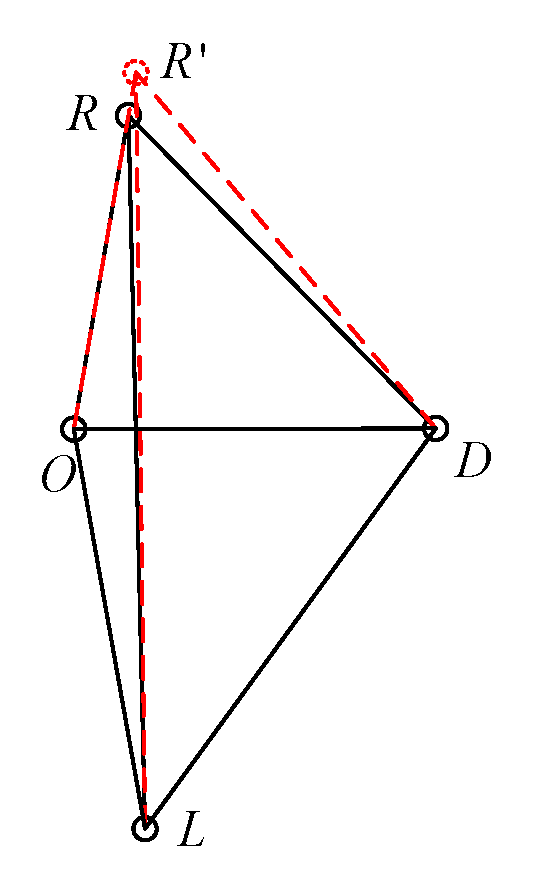
\includegraphics[width=\textwidth]{图片/半径矫正步1.pdf}
        \end{figure}

        \column{0.8\textwidth}
        我们以情况1为例,我们假设$R$和$L$的角度信息都是对的。如果无人机序数$n$为2或者3,我们可以得到:
        \begin{equation}
            \angle LOD = \angle ROD = \frac{2}{9}(n-1)\pi
            \label{eq:上方}
        \end{equation}
        如果无人机序数$n$为8或者9,我们可以得到:
        \begin{equation}
            \angle LOD = \angle ROD = \frac{2}{9}(10-n)\pi
            \label{eq:下方}
        \end{equation}
        由于$OR'=OD$,所以我们可以得到:
        \begin{equation}
            \angle OR'D = \angle ODR' = \frac{\pi - \angle R'OD}{2}
        \end{equation}
    \end{columns}
\end{frame}

\begin{frame}{半径矫正步}
    \begin{columns}
        \column{0.2\textwidth}
        \begin{figure}[!ht]
            \centering
            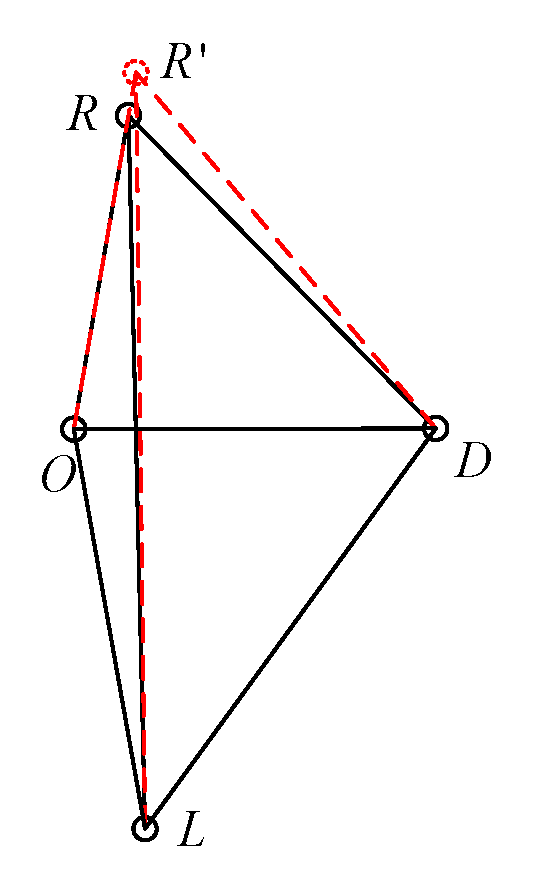
\includegraphics[width=\textwidth]{图片/半径矫正步1.pdf}
        \end{figure}

        \column{0.8\textwidth}
        通过对$\bigtriangleup ORD$使用正弦定理,可以得到:
        \begin{equation}
            OR = \frac{OD\,\sin\left(\pi - \angle ROD - \angle ORD\right)}{\sin \angle ORD}
        \end{equation}
        然后通过对$\bigtriangleup ORL$使用正弦定理,可以得到:
        \begin{equation}
            OL = \frac{OR\,\sin{\angle ORL}}{\sin\left(\pi - \angle ROL - \angle ORL\right)}
        \end{equation}
        其中,$\angle ROL = 2\angle ROD$最后通过对$\bigtriangleup OR'L$使用正弦定理,可以得到方程:
        \begin{equation}
            \frac{OR'}{\sin\left(\pi - \angle ROL - \angle OR'L\right)} = \frac{OL}{\sin\angle OR'L}
        \end{equation}
    \end{columns}
\end{frame}

\begin{frame}{半径矫正步}
    \begin{columns}
        \column{0.2\textwidth}
        \begin{figure}[!ht]
            \centering
            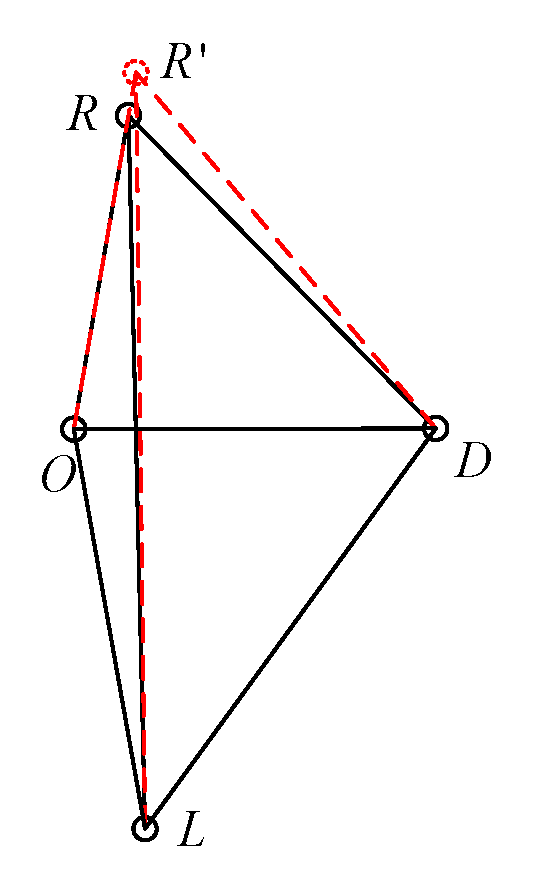
\includegraphics[width=\textwidth]{图片/半径矫正步1.pdf}
        \end{figure}

        \column{0.8\textwidth}
        整理可以得到:
        \begin{equation}
            \frac{\sin\angle ORL\,\sin\left(\angle ROD + \angle ORD\right)\,\sin\left(\angle ROL + \angle OR'L\right)}{\sin\angle ORD\,\sin\left(\angle ROL + \angle ORL\right)\,\sin\angle OR'L} = 1
            \label{eq:初步化简方程}
        \end{equation}
        我们定义$k$为:
        \begin{equation}
            k = \frac{\sin\angle ORL\,\sin\left(\angle ROD + \angle ORD\right)}{\sin\angle ORD\,\sin\left(\angle ROL + \angle ORL\right)}
        \end{equation}
        则式\ref{eq:初步化简方程}可以变为:
        \begin{equation}
            \frac{\sin\left(\angle ROL + \angle OR'L\right)}{\sin\angle OR'L} = \frac{1}{k}
        \end{equation}
    \end{columns}
\end{frame}

\begin{frame}{半径矫正步}
    \begin{columns}
        \column{0.2\textwidth}
        \begin{figure}[!ht]
            \centering
            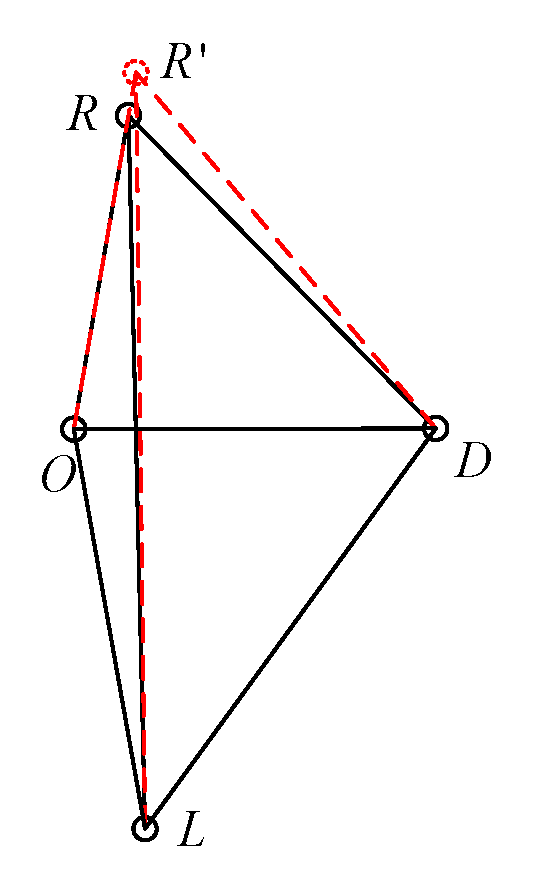
\includegraphics[width=\textwidth]{图片/半径矫正步1.pdf}
        \end{figure}

        \column{0.8\textwidth}
        化简后整理可以得到:
        \begin{equation}
            \angle OR'L = \arctan\frac{\sin\angle ROL}{\frac{1}{k}-\cos\angle{ROL}}
        \end{equation}

        我们依据$\angle OR'L$与$\angle OR'D$的指引,将接收信号的无人机移动到指定位置即可。

        情况2的情况基本类似,$\angle ROD$的计算方式当无人机序数为4和5时同式\ref{eq:上方},当计算无人机序数为6和7时同式\ref{eq:下方},唯一的区别在于$\angle ROL = 2\pi - 2\angle ROD$。
    \end{columns}
\end{frame}

\begin{frame}{调整方案流程}
    我们的调整方案流程如下:
    \begin{enumerate}
        \item 首先选择“半径标定机”,其和原点(及FY00)在之后的调整中不会改变位置;
        \item 重复进行迭代矫正。每次重复时,执行一次“角度矫正轮”,除FY00和“半径标定点”外的所有无人机进行依次“角度矫正步”。如果是第一次执行,还会在“角度矫正轮”前,执行一次“半径矫正轮”,除FY00和“半径标定点”外的所有无人机进行依次“半径矫正步”。
    \end{enumerate}
\end{frame}

\subsection{调整方案的模拟}

\begin{frame}{调整方案的模拟}
    我们在题目给出的信息的基础上,对调整方案进行了模拟。为了衡量无人机组整体位置相对于理想位置的偏差,定义了如下的损失函数:
    \begin{equation}
        L = \sum_{i=0}^{9} d_i^2
    \end{equation}
    其中,$d_i$是序数为$i$的无人机,当前位置与理想位置的欧几里得距离。

    我们还模拟了不采取“半径矫正轮”进行预处理的情况,作为对比,来说明“半径矫正轮”的重要性。
\end{frame}

\begin{frame}{调整方案的模拟}
    无人机在各个阶段的位置如左图所示。损失函数随迭代次数的变化如右图所示。
    \begin{figure}[!ht]
        \centering
        \begin{minipage}[t]{0.32\textwidth}
            \centering
            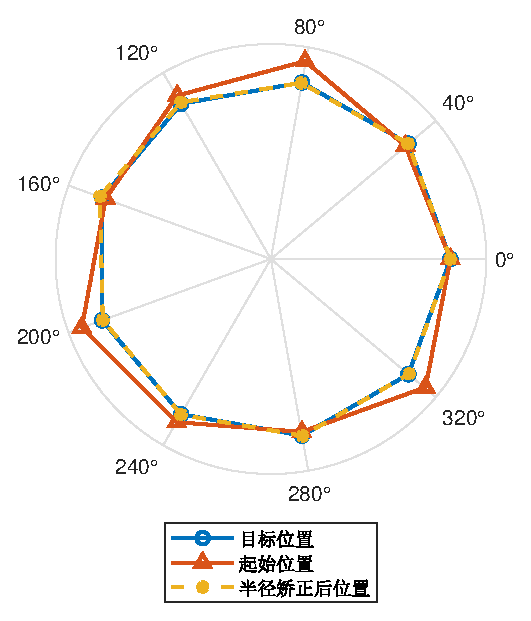
\includegraphics[width=\textwidth]{图片/无人机位置对比.eps}
        \end{minipage}
        \begin{minipage}[t]{0.55\textwidth}
            \centering
            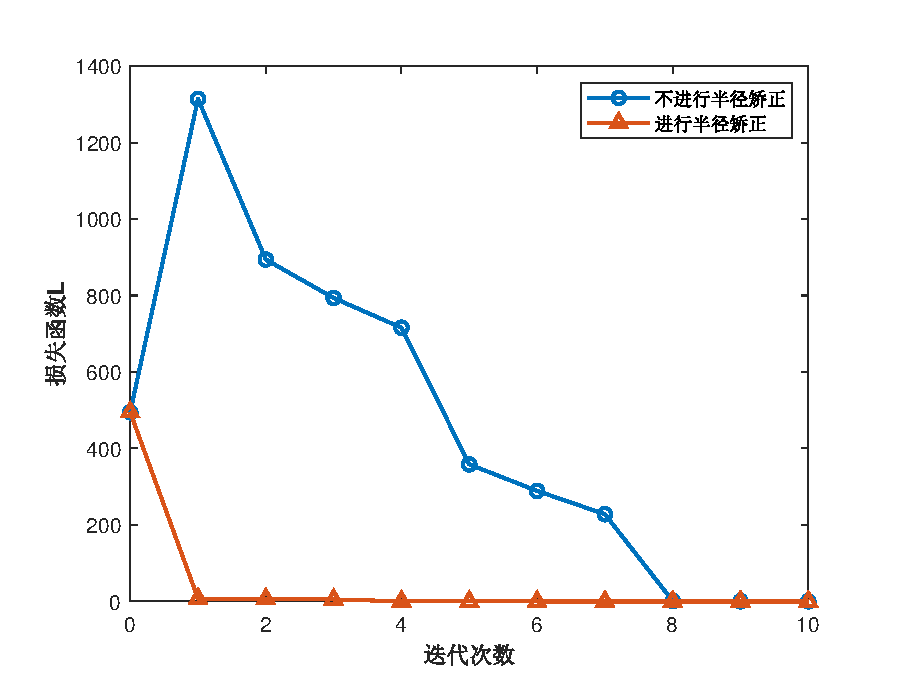
\includegraphics[width=\textwidth]{图片/损失函数变化.eps}
        \end{minipage}
    \end{figure}
\end{frame}

\begin{frame}{调整方案的模拟}
    损失函数的具体数值见下表,损失函数1代表不进行半径矫正时的损失函数,损失函数2代表进行半径矫正时的损失函数。
    \begin{table}[!ht]
        \centering
        \begin{tabular}{ccc|ccc}
            \toprule
            迭代次数 & 损失函数1 & 损失函数2 & 迭代次数 & 损失函数1 & 损失函数2 \\ 
            \midrule
            0 & $4.95\times 10^2$ & $4.95\times 10^2$ & 6 & $2.89\times 10^2$ & $4.04\times 10^{-2}$ \\ 
            1 & $1.31\times 10^3$ & $7.41\times 10^0$ & 7 & $2.28\times 10^2$ & $4.26\times 10^{-5}$ \\ 
            2 & $8.94\times 10^2$ & $6.88\times 10^0$ & 8 & $1.17\times 10^0$ & $3.32\times 10^{-8}$ \\ 
            3 & $7.93\times 10^2$ & $5.28\times 10^0$ & 9 & $6.18\times 10^{-1}$ & $1.98\times 10^{-8}$ \\ 
            4 & $7.16\times 10^2$ & $4.01\times 10^{-1}$ & 10 & $3.51\times 10^{-1}$ & $1.23\times 10^{-8}$ \\ 
            5 & $3.59\times 10^2$ & $8.99\times 10^{-2}$ \\ 
            \bottomrule
        \end{tabular}
    \end{table}
\end{frame}

\begin{frame}{调整方案的模拟}
    \begin{columns}
        \column{0.5\textwidth}
        \begin{figure}[!ht]
            \centering
            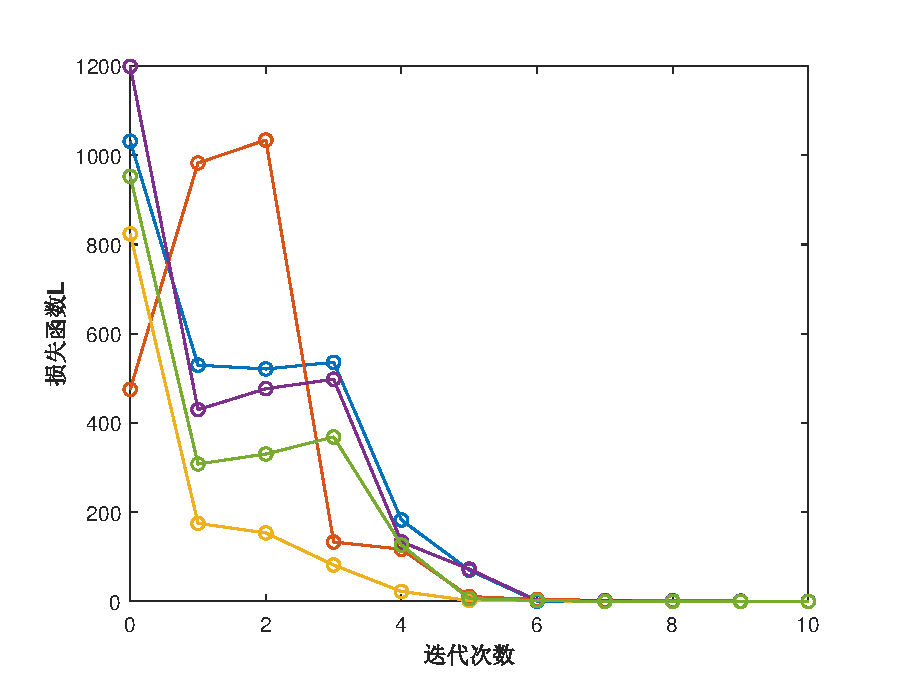
\includegraphics[width=\textwidth]{图片/多次尝试.eps}
        \end{figure}

        \column{0.5\textwidth}
        我们进行了更多的模拟,这些模拟中的数据为随机产生。给除了FY00和FY01外所有的无人机的极坐标角度上加上一个符合$N(0,1)$的偏移,极坐标半径上加上一个符合$N(0,10)$的偏移,这个偏移量远远大于题目中给出的数据的偏移。重新进行了多次模拟,结果如左所示,我们可以看到,我们的策略工作得是非常稳定的。
    \end{columns}
\end{frame}

\subsection{优化后的调整方案}

\begin{frame}{更快收敛的调整策略}
    通过上面的讨论,我们已经已经知道了,三个不共线的位置精确的点,通过两个角度信息,可以确定两个点。若给定任意起始点,其可以沿着梯度方向,到达两个点中的一个。我们知道,对于任何队列来说,其中两个点的位置确定了,整个队列的正确位置就确定了。也就是我们需要使用两个无人机标定这个无人机队列。在这个问题中,我们选择了FY00和FY01。所以我们只需要再确定一个位置精确的点,队列中所有的其他点都可以直接通过角度确定。
\end{frame}

\begin{frame}{更快收敛的调整策略}
    在这个例子中,我们注意到,FY01、FY04和FY07三等分了圆周,我们可以通过类似的迭代方法,使得FY04和FY07的位置逼近正确位置,然后其他无人机的位置就可以直接通过角度确定。这种方法有一下优点:
    \begin{itemize}
        \item 每次调整都有位置正确的FY01参与,可以加速收敛;
        \item 每次迭代都只有2次调整,可以加快迭代速度。
    \end{itemize}
\end{frame}

\begin{frame}{更快收敛的调整策略}
    确定FY01、FY04和FY07位置后,其余无人机可以直接通过与FY04和FY00还有FY07和FY00之间的夹角,直接确定自身位置。我们记一架无人机与FY00和FY04形成的夹角为$\alpha_4$,与FY00和FY07形成的夹角为$\alpha_7$。则其应当调整至的标准角度如下表所示。
    \begin{table}[!ht]
        \centering
        \begin{tabular}{ccc|ccc}
        \toprule
            无人机编号 & $\alpha_4$ & $\alpha_7$ & 无人机编号 & $\alpha_4$ & $\alpha_7$ \\ 
            \midrule
            FY02 & $\frac{5\pi}{18}$ & $\frac{\pi}{18}$ & FY06 & $\frac{5\pi}{18}$ & $\frac{7\pi}{18}$ \\ 
            FY03 & $\frac{7\pi}{18}$ & $\frac{\pi}{18}$ & FY08 & $\frac{\pi}{18}$ & $\frac{7\pi}{18}$\\ 
            FY05 & $\frac{7\pi}{18}$ & $\frac{5\pi}{18}$ & FY09 & $\frac{\pi}{18}$ & $\frac{5\pi}{18}$ \\ 
        \bottomrule
        \end{tabular}
    \end{table}
\end{frame}

\begin{frame}{一些细微的改动}
    圆周上有3个无人机与圆周上有9个无人机调整方案类似,但有些许不同。我们将FY01重新编号为1,FY04重新编号为2,FY7重新编号为3。

    则角度矫正步中理想角度应该改为:
    \begin{equation}
        \alpha_{0NN-1}' = \alpha_{0NN+1}' = \frac{2\pi - \frac{2}{3}\pi}{2} = \frac{1}{6}\pi
    \end{equation}

    半径矫正步中,只会出现情况2,且:
    \begin{equation}
        \angle LOD = \angle ROD = \frac{2}{3}\pi
    \end{equation}
    其余不变。
\end{frame}

\begin{frame}{优化方案的模拟}
    由于我们的方案是在调整好FY04和FY07位置后,其他无人机立刻移动到正确的位置,并不好展现出迭代中逐渐逼近正确位置的过程。我们修改了我们的模拟方案,在FY04和FY07每次迭代调整结束之后,我们都会立即更新所有无人机的位置,然后计算损失函数。
\end{frame}

\begin{frame}{优化方案的模拟}
    我们使用了与左图中相同的起始状态进行模拟,最后得到右图的结果。
    \begin{figure}[!ht]
        \centering
        \begin{minipage}[t]{0.4\textwidth}
            \centering
            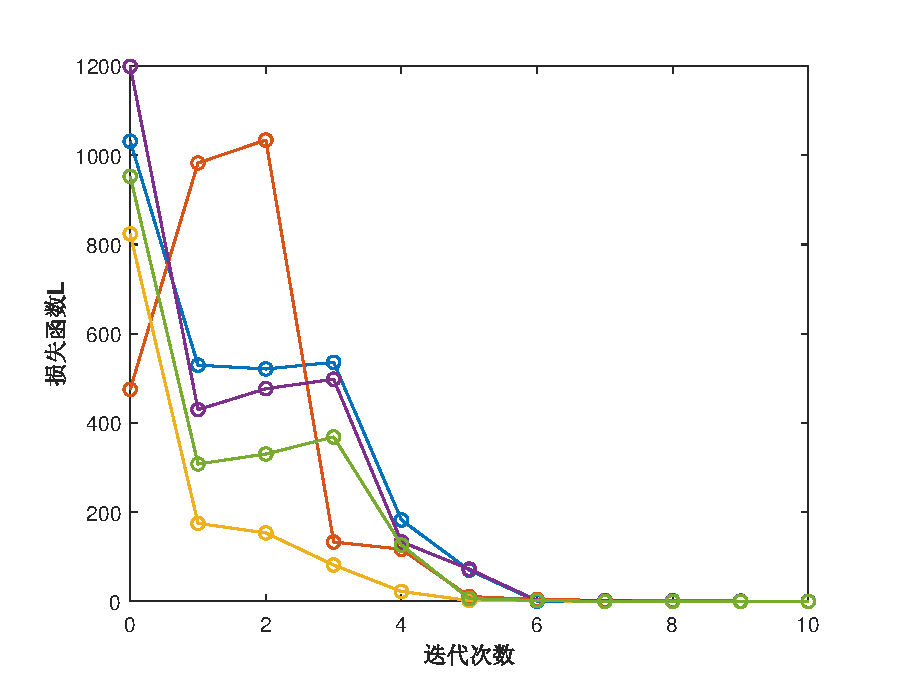
\includegraphics[width=\textwidth]{图片/多次尝试.eps}
        \end{minipage}
        \begin{minipage}[t]{0.4\textwidth}
            \centering
            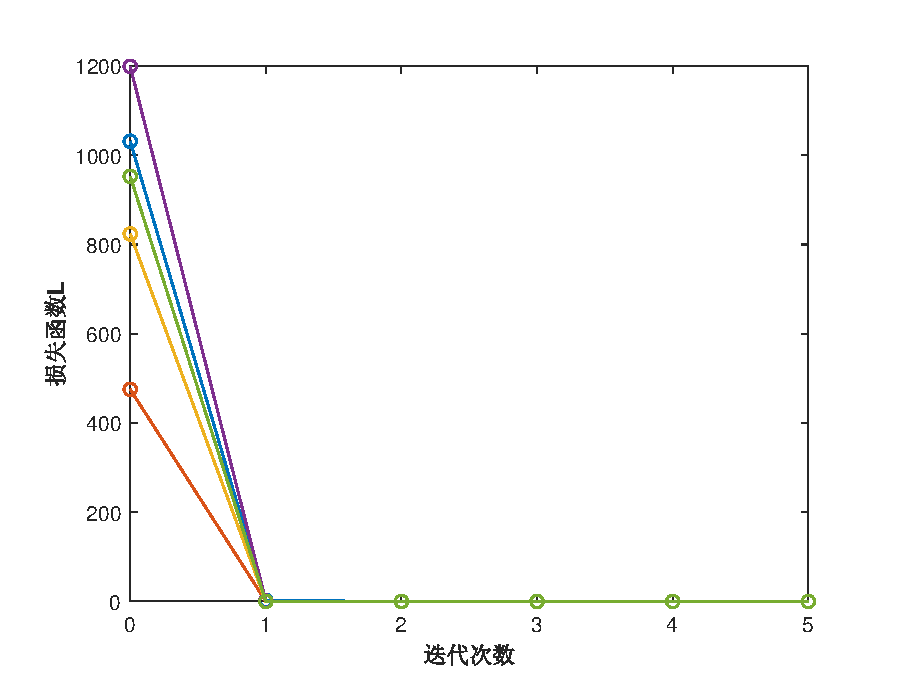
\includegraphics[width=\textwidth]{图片/多次尝试_优化.eps}
        \end{minipage}
    \end{figure}
\end{frame}

%%%%%%%%%%%%%%%%%%%%%%%%%%%%%%%%%%%%%%%%%%%%%%%%%%%%%%%%%%%%%%%%
%                                                              %
%%%%%%%%%%%%%%%%%%%%%%%%%%%%%%%%%%%%%%%%%%%%%%%%%%%%%%%%%%%%%%%%

\section[问题2]{问题二锥形队列调整方案}

\subsection{调整方案}

\begin{frame}{调整方案}
    \begin{columns}
        \column{0.4\textwidth}
        \begin{figure}[!ht]
            \centering
            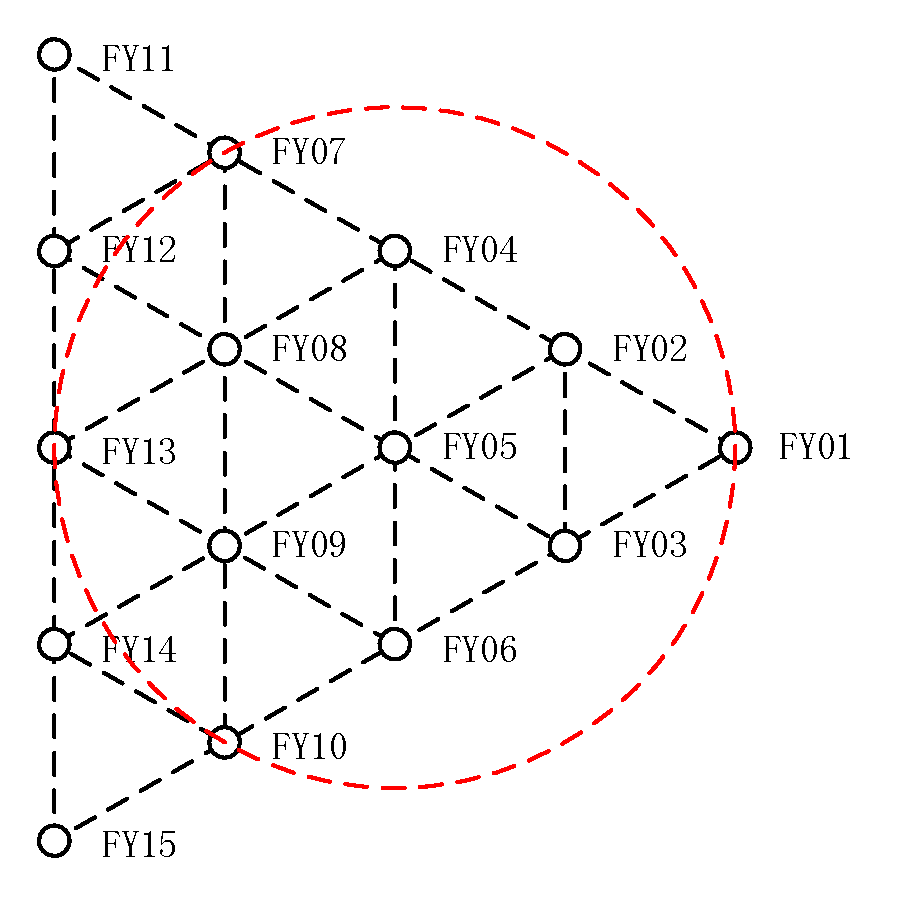
\includegraphics[width=\textwidth]{图片/问题2示意图.pdf}
        \end{figure}

        \column{0.6\textwidth}
        我们沿用上面的策略,考虑对称性,我们选择FY01和FY05的位置来标定无人队列。接下来,我们还需要确定一个位置固定的点。观察左图,我们可以发现,在位置正确的情况下,FY01、FY07和FY10在以FY05为圆心的圆周上,且将圆周三等分。
    \end{columns}
\end{frame}

\begin{frame}{调整方案}
    \begin{columns}
        \column{0.4\textwidth}
        \begin{figure}[!ht]
            \centering
            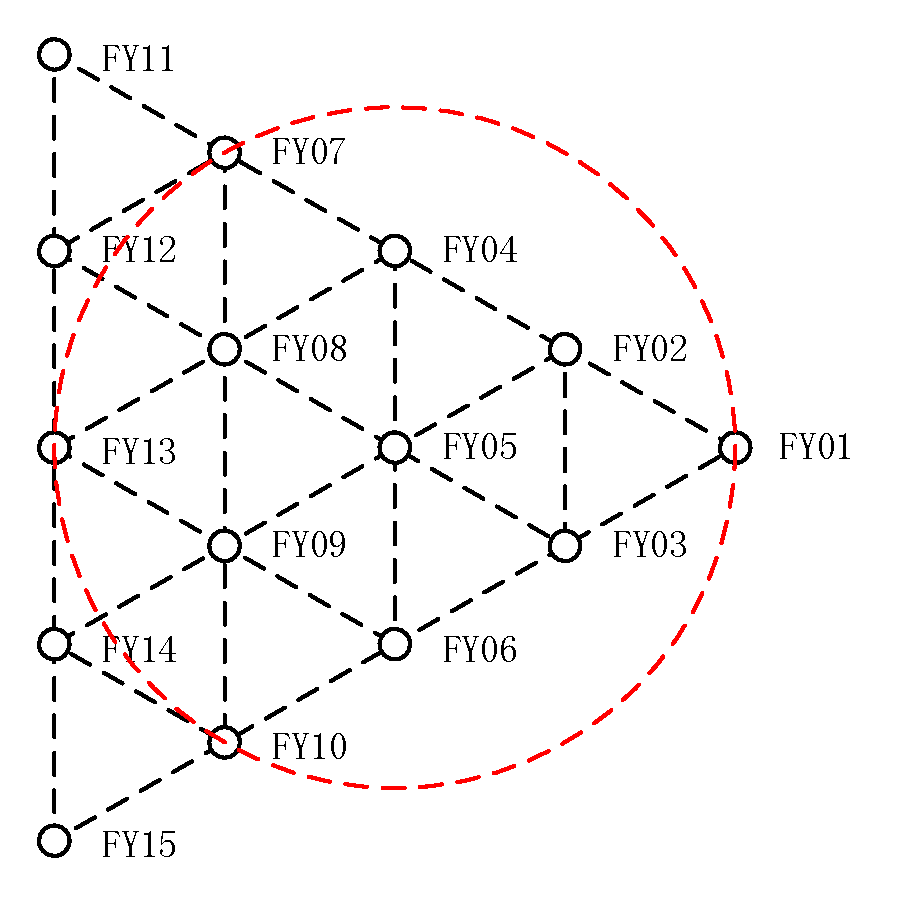
\includegraphics[width=\textwidth]{图片/问题2示意图.pdf}
        \end{figure}

        \column{0.6\textwidth}
        这样,我们就可以给出我们的调整策略:
        \begin{enumerate}
            \item 按照问题一中的策略,将FY01、FY05、FY07和FY10看作一个圆形无人机编队。将FY05作为圆心,FY01作为“半径标定机”。调整FY05和FY07的位置,使其逼近正确位置;
            \item FY05和FY07的位置正确后,其他无人机直接通过与FY07和FY05还有FY10和FY05之间的夹角,直接确定自身位置。
        \end{enumerate}
    \end{columns}
\end{frame}

\begin{frame}{调整方案}
    我们记一架无人机与FY05和FY07形成的夹角为$\alpha_7$,与FY05和FY10形成的夹角为$\alpha_{10}$。则其应当调整至的标准角度如下表所示。
    \begin{table}[!ht]
        \centering
        \begin{tabular}{ccc|ccc}
        \toprule
            无人机编号 & $\alpha_7$ & $\alpha_{10}$ & 无人机编号 & $\alpha_7$ & $\alpha_{10}$ \\ 
            \midrule
            FY02 & $\frac{\pi}{3}$ & $\arctan\frac{\sqrt{3}}{5}$ & FY11 & $\arctan\frac{\sqrt{3}}{5}$ & $\arctan\frac{5\sqrt{3}}{17}$ \\ 
            FY03 & $\arctan\frac{\sqrt{3}}{5}$ & $\frac{\pi}{3}$ & FY12 & $\frac{\pi}{3}$ & $\arctan\frac{\sqrt{3}}{2}$\\ 
            FY04 & $\frac{2\pi}{3}$ & $\arctan\frac{\sqrt{3}}{5}$ & FY13 & $\frac{\pi}{3}$ & $\frac{\pi}{3}$ \\ 
            FY06 & $\arctan\frac{\sqrt{3}}{5}$ & $\frac{2\pi}{3}$ & FY14 & $\arctan\frac{\sqrt{3}}{2}$ & $\frac{\pi}{3}$ \\ 
            FY08 & $\frac{2\pi}{3}$ & $\frac{\pi}{3}$ & FY15 & $\arctan\frac{5\sqrt{3}}{17}$ & $\arctan\frac{\sqrt{3}}{5}$ \\ 
            FY09 & $\frac{\pi}{3}$ & $\frac{2\pi}{3}$ \\ 
        \bottomrule
        \end{tabular}
    \end{table}
\end{frame}

\subsection{调整方案的模拟}

\begin{frame}{调整方案的模拟}
    我们首先将15个无人机的位置设置在正确位置,然后给除了FY01和FY05外所有的无人机加上一个长度随机,方向随机的偏移。这个偏移的长度符合$U\left(0,\frac{S}{2}\right)$,其中$S$为等边三角形的边长。然后我们使用我们的调整方案,将无人机移动到正确的位置。

    同样的,我们修改了我们的模拟方案,在FY07和FY10每次迭代调整结束之后,我们都会立即更新所有无人机的位置,然后计算损失函数:
    \begin{equation}
        L = \sum_{i=1}^{15} d_i^2
    \end{equation}
\end{frame}

\begin{frame}{调整方案的模拟}
    无人机在各个阶段的位置如左图所示。损失函数随迭代次数的变化如右图所示。
    \begin{figure}[!ht]
        \centering
        \begin{minipage}[t]{0.43\textwidth}
            \centering
            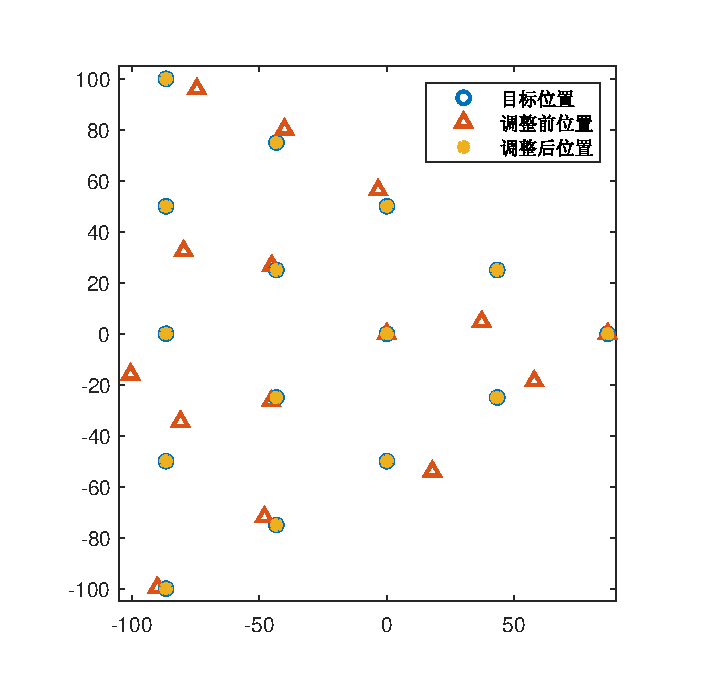
\includegraphics[width=\textwidth]{图片/无人机位置对比_锥形.eps}
        \end{minipage}
        \begin{minipage}[t]{0.55\textwidth}
            \centering
            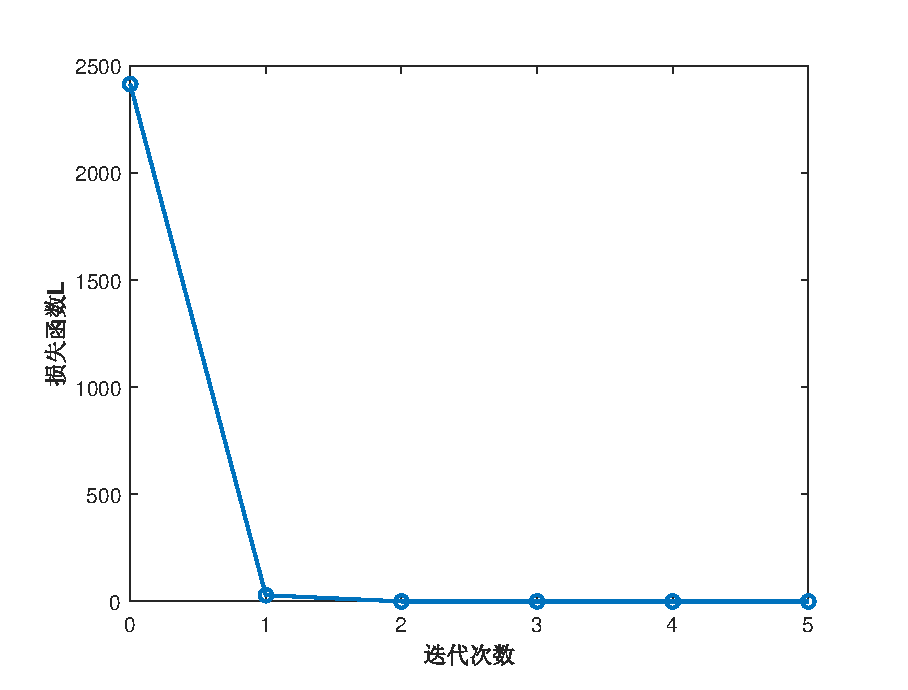
\includegraphics[width=\textwidth]{图片/损失函数变化_锥形.eps}
        \end{minipage}
    \end{figure}
\end{frame}

\begin{frame}{调整方案的模拟}
    损失函数的具体数值见下表所示。
    \begin{table}[!ht]
        \centering
        \caption{锥形队列损失函数变化情况}
        \label{tab:损失函数变化_锥形}
        \begin{tabular}{cc|cc}
            \toprule
            迭代次数 & 损失函数 & 迭代次数 & 损失函数 \\
            \midrule
            0 & $2.41\times 10^3$ & 3 & $3.70\times 10^{-10}$ \\ 
            1 & $2.91\times 10^1$ & 4 & $3.70\times 10^{-10}$ \\ 
            2 & $3.70\times 10^{-10}$ & 5 & $3.70\times 10^{-10}$ \\ 
            \bottomrule
        \end{tabular}
    \end{table}
    我们从中可以看出,我们的对于锥形队列无人机的调整方案也非常有效,可以很好地将无人机固定在正确的位置。
\end{frame}

%%%%%%%%%%%%%%%%%%%%%%%%%%%%%%%%%%%%%%%%%%%%%%%%%%%%%%%%%%%%%%%%
%                                                              %
%%%%%%%%%%%%%%%%%%%%%%%%%%%%%%%%%%%%%%%%%%%%%%%%%%%%%%%%%%%%%%%%

\section[评价、改进、推广]{模型的评价、改进与推广}

\begin{frame}{模型优点}
    我们的模型具有以下优点:
    \begin{itemize}
        \item 在第一问第1小问中,我们的基于两圆相交的定位模型,可以给出待定位无人机位置的解析解;
        \item 在第一问第2小问中,我们基于严格的数学证明,证明了在待定无人机的位置偏差满足式\ref{eq:误差条件}的情况下,通过额外两架无人机发射的信号,就可以确定待定无人机的位置;
        \item 在第一问第2小问中,我们还讨论了一架额外无人机就可以确定待定无人机位置的情况;
        \item 在第一问第3小问中,我们提出了一种基于迭代的调整方案,可以使得无人机队列快速逼近正确位置,并且给出了收敛更快的优化后的调整策略;
        \item 在第二问中,我们将其转化为了与第一问相似的问题,并进行了解决。
    \end{itemize}
\end{frame}

\begin{frame}{模型缺点}
    我们的模型还具有以下不足:
    \begin{itemize}
        \item 我们的模型对于误差范围更加极端的情况,适应性较差;
        \item 对于第二问,没有讨论待定无人机位置偏差不满足式\ref{eq:误差条件}的情况。
    \end{itemize}
\end{frame}

\begin{frame}{模型改进方向}
    我们可以考虑如下的改进思路:
    \begin{itemize}
        \item 可以考虑无人机之间可以互相通信的情况;
        \item 可以考虑无人机按非中心对称的方式排列的情况;
        \item 可以考虑三维情况下的无人机定位问题;
    \end{itemize}
\end{frame}

\begin{frame}{模型推广}
    我们的模型实际上并没有使用无人机所特有的性质,其可以推广到所有需要进行二维平面无源定位的情况。
\end{frame}

\appendix

\begin{frame}
    \begin{center}
        {\Huge\calligra Thanks!}
    \end{center}
\end{frame}

\end{document}